\documentclass[12pt]{report}

% Style
\usepackage{parskip}	% Blank line between paragraphs
\usepackage[top=1in, bottom=1.25in, left=1.25in, right=1.25in]{geometry} % Page margins
\usepackage{float} % Placement of figures with H
\renewcommand{\familydefault}{\sfdefault} % Use sans-serif font (https://tex.stackexchange.com/a/2097)

% Maths
\usepackage{graphicx}
\usepackage{amsmath}
\usepackage{amssymb}
\usepackage{units}
\usepackage{relsize}    % \mathlarger

\usepackage[hidelinks, pdfusetitle]{hyperref}
\usepackage{color}

% Settings
% \allowdisplaybreaks		% Break aligned equations over pages

% Parameters
\newcommand{\version}{0.8}
\newcommand{\website}{\href{http://www.virtualbow.org/}{\texttt{\textcolor{blue}{http://www.virtualbow.org/}}}}
\newcommand{\copyrights}{Copyright (C) 2016-2020 Stefan Pfeifer}

\begin{document}

\begin{titlepage}

\vspace*{5em}
\centering{\Huge\textbf{\swtitle~v\version \\[1em] Theory Manual}}

\vspace{5em}

\centerline{
\includegraphics[width=0.2\textwidth]{figures/logo.png}}

\thispagestyle{empty}
\end{titlepage}


\tableofcontents

\chapter{Introduction}

This is the theory manual for \swtitle, an open-source software tool for simulating bow and arrow physics.
For the latest version of the software and this document visit

\website.

This documentation, as opposed to the user manual, is about the theoretical foundations and technical details of the software.
It is meant as a reference for developers and interested users.
\chapter{The Bow Model}

A scientific model is a simplification and abstraction of reality, often formulated in a mathematical way.
A good model reduces the complexity of a real system by including only its most significant aspects and disregarding less significant ones.
The results of analyzing this simplified model can then be used to draw conclusions about the real system.

What aspects of reality a model has to reflect depends on the kinds of questions it seeks to answer.
The first step for developing a bow model is therefore to clarify its scope and intended application.

\section{Scope of the Model}
\label{section:model-scope}

In the case of \swtitle\ the purpose of the bow model is to give users the ability to evaluate the bow designs they come up with.
So what characteristics make a bow design a good one and what are their implications for the bow model?
Many things come to mind, but we limit ourselves to the following three categories:

\begin{enumerate}
\item \textbf{Viability}: Can the design be realised? Do the materials withstand the arising loads when the bow is being used?
To be able to judge this the model has to accurately predict the distribution of stress across the limbs as well as the tensile forces in the string that arise when drawing and shooting the bow.

\item \textbf{Performance}: Important performance characteristics are the arrow's velocity, kinetic energy and the bow's degree of efficiency, i.e. the percentage of the stored elastic energy that is converted into kinetic energy of the arrow during the shot.
To capture these things the model has to reflect all major mechanisms of efficiency loss in a bow.
We will later see what those are when we look at scientific research.

\item \textbf{Comfort}: Viability and raw performance aren't everything.
A bow design will also be judged by it's influence on the archer, like the draw force, the shape of the draw curve (no "stacking", i.e. increasing stiffness towards the end of draw) and the dynamic forces exerted to the shooter ("hand shock").
\end{enumerate}

Any physical effects in archery that don't (significantly) affect one of those categories above are outside the scope of \swtitle\ and the bow model doesn't need to include them.
Exterior ballistics is an example for this, another one is the bending motion of the arrow (Archer's Paradox).

Now the next question is: How does a bow model have to look like in order to capture the things listed above?
That's not easy to answer, but luckily there has been done quite some scientific research about bow and arrow physics in the past, so we don't have to start completely from scratch.
The next section therefore examines some of that research before we define our own model.

\section{Literature Review}

Research about the mechanics of bow and arrow goes back to at least the 1930s, when C.N.~Hickman, P.E.~Klopstek and others performed systematic experiments and developed simple mathematical models.
Without modern computers available these early models were still limited in their complexity by what could be solved analytically.
The focus was therefore more on qualitative insight rather than accurate prediction.
One of those early models is the~\textit{Hickman Model}~\cite{bib:hi37}, published in~1937.
It assumes two rigid limbs that are connected to the stationary rest of the bow via elastic hinges as shown in figure~\ref{fig:model:hickman}.
Even though this is a huge simplification, this model can already be used to investigate the efficiency of a bow, i.e. how it transfers its stored elastic energy to an arrow.

\begin{figure}[h]
\centering
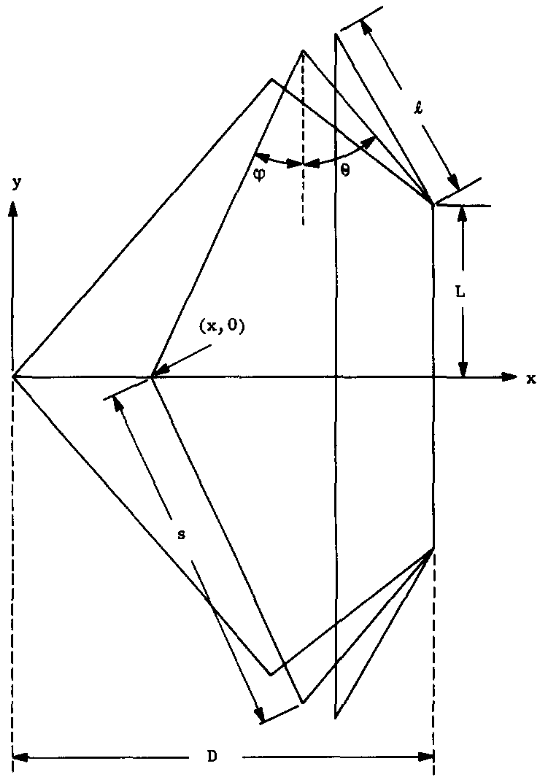
\includegraphics[width=0.4\textwidth]{figures/model/hickman}
\caption{Hickman model as used by W.C. Marlow \cite{bib:ma80}}
\label{fig:model:hickman}
\end{figure}

An important modification to the Hickman model was suggested by W.C.~Marlow in 1980~\cite{bib:ma80}.
It was already well-known that the original Hickman model with an inextensible string severely overpredicted a bow's degree of efficiency.
(Predicted efficiencies typically over 90\% while measurements suggest values between 70\% and 85\% for most bows.)
Popular explanations for this discrepancy were effects like hysteresis and air resistance.
Marlow however found another reason: With an inextensible string (as in Hickman's original model) the arrow exits the bow exactly at brace height, where the limbs have zero velocity.
Only the kinetic energy of the string remains in the bow, the rest is transferred to the arrow.
Marlow then showed that accounting for the elasticity of the string shifts the point of exit for the arrow away from the braced position, such that the limbs still have substantial kinetic energy left. In his numerical example the modification reduces the predicted efficiency to~78\% as opposed to~92\% previously.
Of the energy remaining in the bow,~11\% were the kinetic energy of the limbs,~9\% the kinetic energy of the string and~2\% the potential energy of limbs and string.

This leads to an important realization: The efficiency of a bow is mainly determined by the kinetic energy that stays in the system due to mass and elasticity of the string and the mass distribution of the limbs. The contribution of dissipative effects like air resistance and hysteresis to the overall efficiency was estimated by Marlow to be less than~2\% and~3\% respectively.

The widespread availability of digital computers eventually made it possible to simulate much more detailed models and therefore make more accurate predictions.
Much notable work in this area has been done by Dr.~Bob~Kooi and his co-authors.
Over the course of the~1980s and~90s they published a good amount of papers about the mechanics of bow and arrow in which they utilize numerical methods to solve increasingly complex mathematical models.

The first one of those papers is titled \textit{On the static deformation of a bow}~\cite{bib:kosp80} and investigates the storage of deformation energy in bows with and without recurve. Figure~\ref{fig:model:kooi} shows the model used there.
The bow is assumed to be symmetric and has an inextensible string.
The limbs are represented by an Euler-Bernoulli beam, which is an infinitely thin, elastic line with a certain (varying) bending stiffness for which the Euler-Bernoulli assumptions hold.
These are assumptions about the kinematics of the deformation, namely that the cross sections of the beam always stay flat and perpendicular to its centerline. This is typically a good approximation for slender beams, that is beams whose length is much larger than their cross section dimensions. Kooi uses the general version of the Euler-Bernoulli equation that accounts for arbitrarily large deformation. Combining this with geometric constraints for the string and some boundary conditions leads to the bow's equations of equilibrium, a free-boundary value problem for a set of ordinary differential equations. The equations of equilibrium are solved numerically for specific draw lengths of the bow.

\begin{figure}[h]
\centering
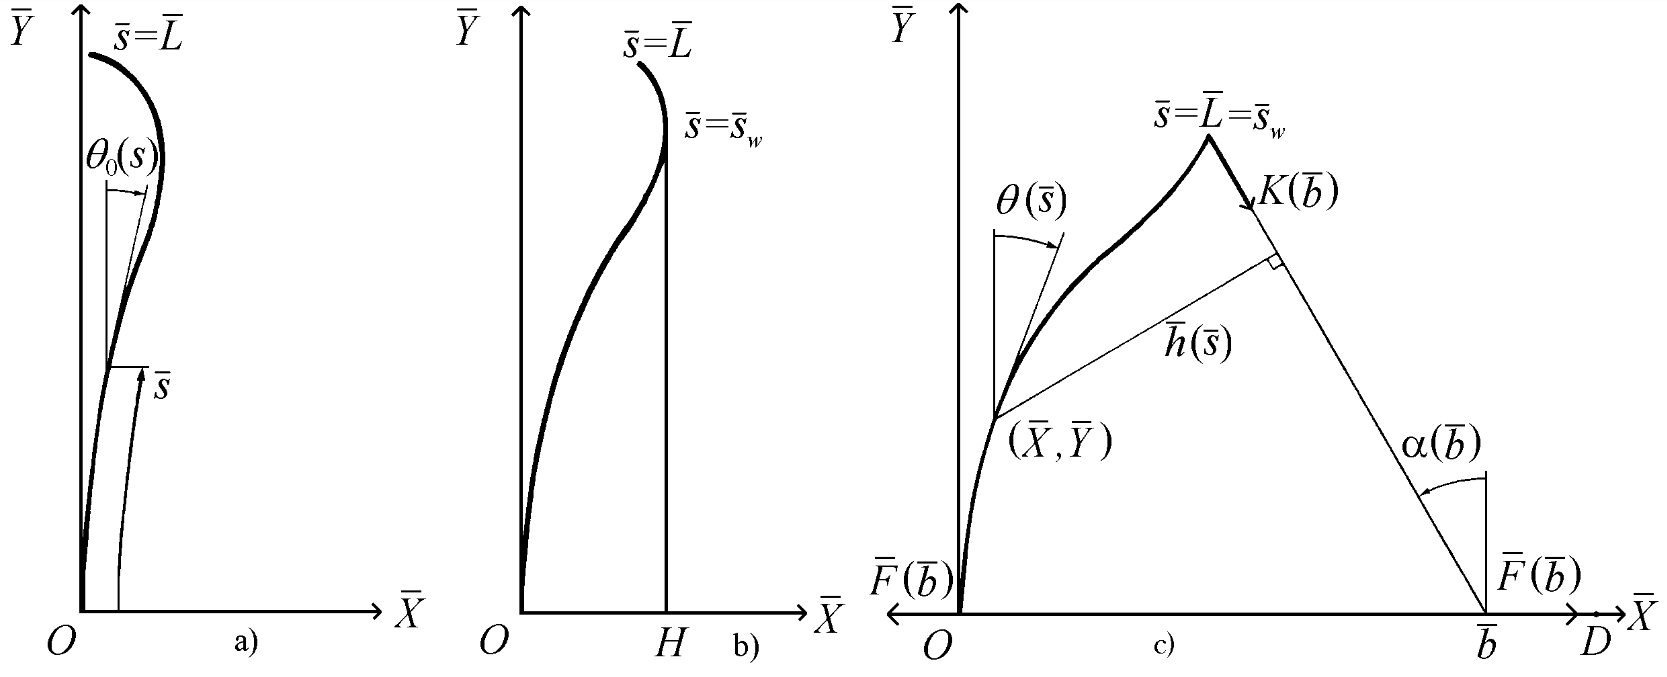
\includegraphics[width=0.8\textwidth]{figures/model/kooi}
\caption{Bow model used by Bob Kooi \cite{bib:kosp80}}
\label{fig:model:kooi}
\end{figure}

In subsequent papers titled \textit{On the mechanics of the bow and arrow}~\cite{bib:kooi81} and \textit{On the mechanics of the modern working-recurve bow}~\cite{bib:kooi91} Kooi also considers the dynamic case. Like Marlow he uses a linear-elastic string and assumes the arrow as a concentrated point mass. The equations of motion for the system form a moving-boundary value problem for a set of partial differential equations. They are solved numerically by using a finite-difference method with complete discretization. (Both space and time are approximated by a discrete "grid" of values. The partial derivatives in the governing equations are then approximated by finite difference quotients operating on those grid values. The resulting large number of difference equations can then be solved with a computer program.)

In the paper \textit{On the Mechanics of the Arrow: Archer's Paradox}~\cite{bib:kosp97}, Kooi refines his model even more by including an elastic arrow with a sliding contact to the bow's grip. This makes it possible to analyze the Archer's Paradox: The phenomenon of arrows going around the grip of a bow by performing a bending motion in the horizontal plane. The dynamics of the arrow are however treated partly decoupled from the bow's dynamics: Only the influence of the bow on the arrow's motion is considered, the other way around is neglected. This is in line with our assumption from section~\ref{section:model-scope} that the bending motion of the arrow doesn't contribute much to a bow's overall performance and is therefore out of scope for our model.

\section{Model Definition}

We have now learned enough in order to define our own bow model. First of all a few words on the general modeling approach. As we saw in the previous section, any decently complex bow model cannot be solved analytically but has to be combined with some sort of numerical method for calculating an approximate solution. Models based on continuum mechanics (e.g. Euler-Bernoulli beam theory) always have an infinite number of degrees of freedom and will eventually have to be approximated by a discrete system with finitely many degrees of freedom in order to be solvable by a computer program. This step is called discretization. Kooi for example, like a true mathematician, formulates the complete equations of motion for his continuous bow model and only then starts to employ a discretization technique (in this case a finite difference method) to solve those equations. This results in a clear separation between the mathematical model and the numerical solution methods.

We're going to use more of an engineering approach here instead and start with a discrete system in the first place. We do this by constructing the continuous parts of the bow from a large number of so-called finite elements. A finite element is an approximation of a little part of a continuous structure, e.g. a beam or a bar, but with only finitely many degrees of freedom, namely the displacements of the nodes at which the elements are connected to each other. The more elements are used, the better the approximation gets and the closer the results will be to the exact solution.

The finite element method leads to a (potentially large) system of ordinary differential equations as the equations of motion, which can be solved by standard numerical methods as we will see later.

\begin{figure}[h]
\centering

\includegraphics[width=0.8\textwidth]{figures/model/bow-simulator}
\caption{Finite element model of the bow}
\label{fig:model:bow-simulator}
\end{figure}

Figure~\ref{fig:model:bow-simulator} shows the finite element approximation of our bow model. Like Kooi's model it is symmetric with respect to the horizontal plane, assumes the limbs to satisfy the Euler-Bernoulli assumptions and neglects any dissipative effects like air resistance and hysteresis. The limbs are therefore made up of Euler-Bernoulli beam elements. A concentrated point mass is placed at the tips to account for any added weight, like overlays for example.

The string, as opposed to the limbs, only transfers longitudinal forces and is therefore approximated by linear-elastic bar elements. We limit ourselves to linear elasticity for pragmatic reasons: Obtaining the exact nonlinear stress-strain curve of a particular string material is pretty difficult. Instead, any material nonlinearity (which can be the case especially for modern synthetic materials) will have to be accounted for by using an "average" stiffness. In the previous section we saw that the mass properties of the string are fairly important, so in addition to the mass of the string itself there are two additional point masses at the tips and center to account for things like servings, nocking point, etc.

The arrow is another point mass, as already justified earlier. It is connected to the string by an ideal, frictionless contact without any release force. This means that the arrow will be released as soon as the string doesn't push against/accelerate it anymore.

Not shown in figure~\ref{fig:model:bow-simulator} are the contact elements that prevent the string nodes from passing through the limb, thereby making it possible to simulate recurves. These are also ideal contacts without any friction.

All in all, there are four different types of elements needed:

\begin{itemize}
\item Beam Elements (Limbs)
\item Bar Elements (String)
\item Mass Elements (Arrow + additional masses)
\item Contact Elements (String to limb contact)
\end{itemize}

All of them have to account for arbitrarily large displacements and are therefore geometrically nonlinear (even though all the materials are linear-elastic).

In the next chapters we will first show how the equations of motion for a finite element system can be assembled from the equations of motion for the single elements. We will then derive the equations of motion for the element types listed above. Finally we're going to discuss the numerical solution of those equations for the static and dynamic case and how this is implemented in \swtitle.
\chapter{Equations of Motion}

Consider a single, unconstrained finite element~$i$ with~$n$ degrees of freedom.
Its configuration at time~$t$ will be described by the displacement vector~$\boldsymbol{u}_i(t) \in \mathbb{R}^n$ containing all positions and rotation angles of the nodes.
The equation of motion for the kind of elements we're concerned with takes the form

\begin{equation}
\boldsymbol{M}_i\,\ddot{\boldsymbol{u}}_i + \boldsymbol{q}_i(\boldsymbol{u}_i,\,\dot{\boldsymbol{u}}_i) = \boldsymbol{p}_i(t).\label{eq:local-equation-of-motion}
\end{equation}

This is a nonlinear ordinary differential equation of second order for the displacements.
$\boldsymbol{M}_i \in \mathbb{R}^{n \times n}$ is called the element's mass matrix,~$\boldsymbol{q}_i \in \mathbb{R}^n$ is the vector of internal forces depending on the displacements and their associated velocity (e.g. elastic forces, damping forces, \ldots) and~$\boldsymbol{p}_i \in \mathbb{R}^n$ is the vector of externally applied loads.

Now consider a finite element system that consists of a number of such elements that are connected to each other in a certain way.
If the overall system has a total of~$N$ degrees of freedom, it's configuration can be described by the global displacement vector~$\boldsymbol{u}(t) \in \mathbb{R}^{N}$.
The local element displacements~$\boldsymbol{u}_i$ are now no longer independent but instead directly related to the global displacements of the system they are part of.
In our case these relationships can be written as

\begin{equation}
\boldsymbol{u}_i = \boldsymbol{T}_i\,\boldsymbol{u},\label{eq:kinematics-local-global}
\end{equation}

where~$\boldsymbol{T_{i}} \in \mathbb{R}^{\mathlarger{n} \times N}$ is a constant transformation matrix for the respective element.
Using the local equations of motion~(\ref{eq:local-equation-of-motion}), the kinematic relationship~(\ref{eq:kinematics-local-global}) and some analytical mechanics it can be shown \textcolor{red}{[add citation]} that the equation of motion of the overall system takes the similar form

\begin{equation}
\boldsymbol{M}\,\ddot{\boldsymbol{u}} + \boldsymbol{q}(\boldsymbol{u},\,\dot{\boldsymbol{u}}) = \boldsymbol{p}(t).
\end{equation}

where the global mass matrix $\boldsymbol{M} \in \mathbb{R}^{N \times N}$, internal forces~$\boldsymbol{q} \in \mathbb{R}^{N}$ and external forces $\boldsymbol{p} \in \mathbb{R}^{N}$ are calculated from the local element matrices as

\begin{align}
\boldsymbol{M} &= \sum_i\boldsymbol{T}_i^\mathsf{T}\, \boldsymbol{M}_i\,\boldsymbol{T}_i,\\
\boldsymbol{q} &= \sum_i\boldsymbol{T}_i^\mathsf{T} \boldsymbol{q}_i(\boldsymbol{T}_i\,\boldsymbol{u},\,\boldsymbol{T}_i\,\dot{\boldsymbol{u}}),\\
\boldsymbol{p} &= \sum_i\boldsymbol{T}_i^\mathsf{T}\,\boldsymbol{p}_i.
\end{align}

In practice, because of the way the element displacements are related to the overall displacements, the transformation matrices~$\boldsymbol{T}_i$ only contain ones and zeros, effectively describing a selection of entries.
Therefore it is not actually necessary to carry out all the matrix multiplications occurring above.
Instead, the entries of the local matrices can be directly added to the corresponding entries of the global matrices.

In order to solve the equations of motion for equilibrium we're later going to need the derivative of the internal forces with respect to the displacements, which is called the tangent stiffness matrix~$\boldsymbol{K} \in \mathbb{R}^{N \times N}$ of the system,

\begin{equation}
\boldsymbol{K}(\boldsymbol{u}) = \frac{\partial \boldsymbol{q}}{\partial \boldsymbol{u}}
\end{equation}

It can be calculated from the element's local tangent stiffness matrices~$\boldsymbol{K}_i = \frac{\partial \boldsymbol{q}_i}{\partial \boldsymbol{u}_i}$ like this,

\begin{align*}
\boldsymbol{K}(\boldsymbol{u}) &= \frac{\partial \boldsymbol{q}}{\partial \boldsymbol{u}} = \sum_i\boldsymbol{T}_i^\mathsf{T} \frac{\partial \boldsymbol{q}_i}{\partial \boldsymbol{u}} = \sum_i\boldsymbol{T}_i^\mathsf{T} \frac{\partial \boldsymbol{q}_i}{\partial \boldsymbol{u}_i} \frac{\partial \boldsymbol{u}_i}{\partial \boldsymbol{u}} = \sum_i\boldsymbol{T}_i^\mathsf{T} \frac{\partial \boldsymbol{q}_i}{\partial \boldsymbol{u}_i} \boldsymbol{T}_i\\
&= \sum_i\boldsymbol{T}_i^\mathsf{T} \boldsymbol{K}_i \boldsymbol{T}_i.
\end{align*}

For now this is all we have to know about the equations of motion of the finite element system.
What's going to be needed next are the local equations of motion for the different element types.
Those are going to be derived in the next sections.

\newpage
\section{Mass Element}

The point mass is the most simple element.
Figure~\ref{fig:elements:point-mass} shows its definition: A mass~$m$ is placed in a cartesian coordinate system. Its position is described by the displacements~$u_0(t)$ and~$u_1(t)$ along the coordinate axes.
The external forces~$p_0(t)$ and~$p_1(t)$ are acting in the direction of the respective displacements.

\begin{figure}[h]
\centering
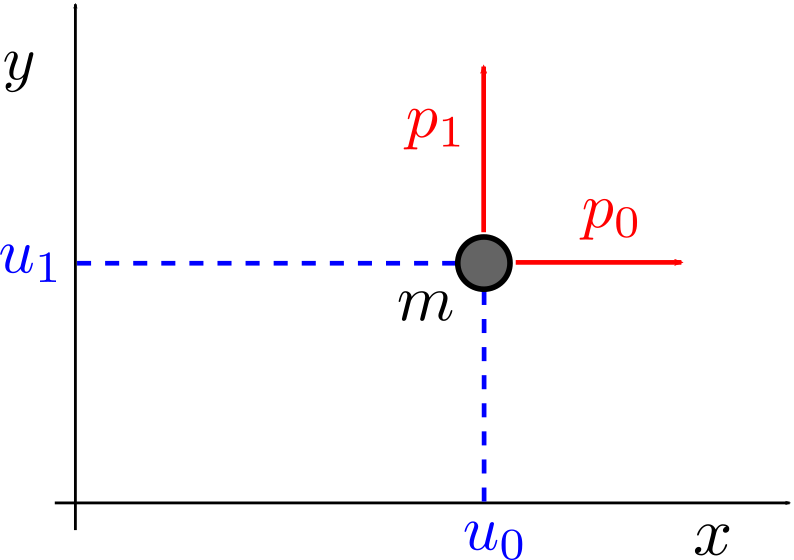
\includegraphics[width=0.4\textwidth]{figures/elements/mass-element}
\caption{Point mass element}
\label{fig:elements:point-mass}
\end{figure}

The equation of motion for this system can be written down directly by using Newton's second law of motion:

\begin{equation}
\underbrace{
\begin{bmatrix}
m & 0\\
0 & m
\end{bmatrix}
}_{\boldsymbol{M}}
\underbrace{
\begin{bmatrix}
\ddot{u}_0\\
\ddot{u}_1
\end{bmatrix}
}_{\boldsymbol{\ddot{u}}}
+
\underbrace{
\begin{bmatrix}
0\\
0
\end{bmatrix}
}_{\boldsymbol{q}(\boldsymbol{u},\,\dot{\boldsymbol{u}})}
=
\underbrace{
\begin{bmatrix}
p_0\\
p_1
\end{bmatrix}
}_{\boldsymbol{p}(t)}
\end{equation}

This immediately gives us the element's mass matrix, internal forces (which are zero) and external forces.
Because the internal forces are zero, the tangent stiffness matrix is zero as well:

\begin{equation}
\boldsymbol{K} = \frac{\partial \boldsymbol{q}}{\partial \boldsymbol{u}} =
\begin{bmatrix}
0 & 0\\
0 & 0
\end{bmatrix}.
\end{equation}

\newpage
\section{Bar Element}

A bar only transfers forces in longitudinal direction, it has no bending stiffness. Figure~\ref{fig:bar-element-1} shows a bar with an initial length of~$L$ that is subjected to a normal force~$N$ which causes it to elongate by~$\Delta L$.

\begin{figure}[h]
\centering
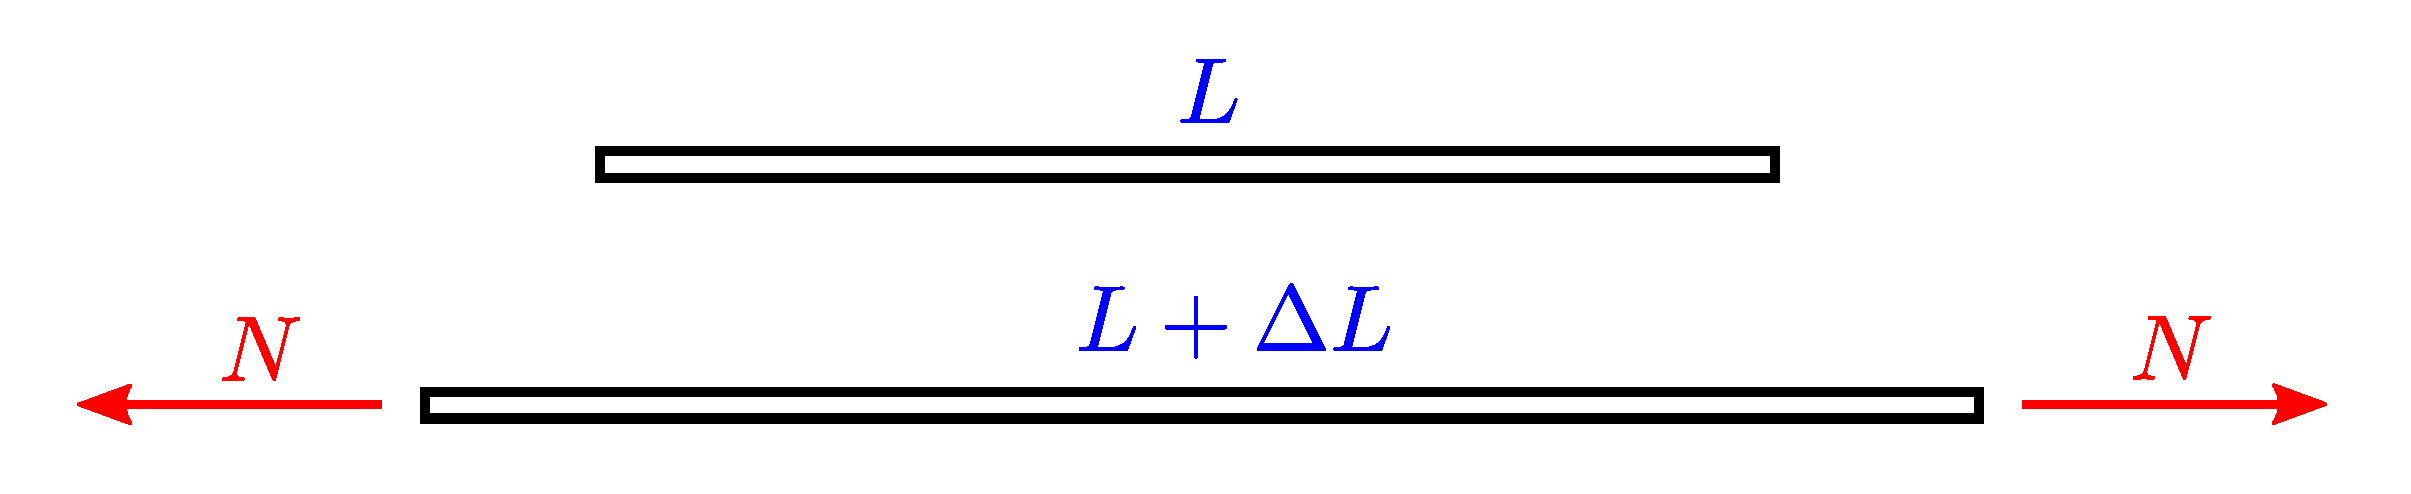
\includegraphics[width=0.75\textwidth]{figures/elements/bar-element-1}
\caption{Elongation of a bar under load}
\label{fig:bar-element-1}
\end{figure}

For a linear-elastic bar with constant cross section area~$A$ and elastic modulus~$E$ the constitutive relationship that connects force and elongation is

\begin{equation}
N = EA\,\frac{\Delta L}{L}.\label{eq:bar-constitutive}
\end{equation}

The product~$EA$ is also called the longitudinal stiffness. The bar is now placed between the two nodes A and B as shown in figure~\ref{fig:bar-element-2}. Its configuration is described by the nodal displacements~$\boldsymbol{u} = (u_0,\,u_1,\,u_2,\,u_3)^\mathsf{T}$.

\begin{figure}[h]
\centering
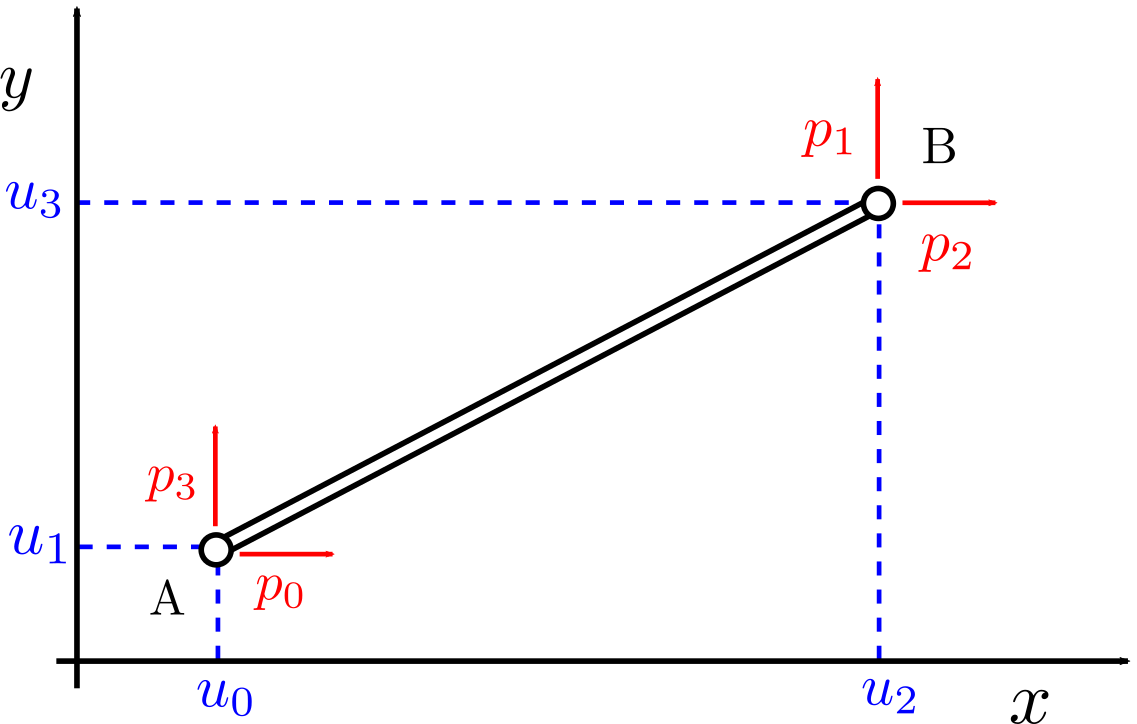
\includegraphics[width=0.6\textwidth]{figures/elements/bar-element-2}
\caption{Bar element}
\label{fig:bar-element-2}
\end{figure}

The position vectors of the two nodes are given by

\begin{equation}
\boldsymbol{r}_A =
\begin{bmatrix} u_0 \\ u_1 \end{bmatrix}, \quad
\boldsymbol{r}_B =
\begin{bmatrix} u_2 \\ u_3 \end{bmatrix}.\label{bar:node-positions}
\end{equation}

The mass of the element is assumed to be concentrated at the nodes, so that each of them is carrying half of the total mass.
This is called a lumped mass approach and will later lead to a constant, diagonal mass matrix.
For a bar with density~$\rho$ the mass of a node is therefore~$\frac{1}{2}\rho A L$. With this in mind we can write down Newton's second law of motion for each of the two nodes,

\begin{align}
\frac{\rho A L}{2}\,\ddot{\boldsymbol{r}}_A = \boldsymbol{q}_A + \boldsymbol{p}_A,\label{eq:bar-newton-1}\\
\frac{\rho A L}{2}\,\ddot{\boldsymbol{r}}_B = \boldsymbol{q}_B + \boldsymbol{p}_B.\label{eq:bar-newton-2}
\end{align}

Here,~$\boldsymbol{q}_A$,~$\boldsymbol{q}_B$ are the elastic forces that the bar exerts to the respective nodes and~$\boldsymbol{p}_A$,~$\boldsymbol{p}_B$ are the externally applied loads. The elastic forces can be obtained by multiplying the scalar normal force~$N$ in the bar~(\ref{eq:bar-constitutive}) with the tangent vector of the connecting line between the two nodes to account for the direction,

\begin{align}
\boldsymbol{q}_A &= N\,\frac{\boldsymbol{r}_B - \boldsymbol{r}_A}{|\boldsymbol{r}_B - \boldsymbol{r}_A|} = EA\,\frac{\Delta L}{L}\, \frac{\boldsymbol{r}_B - \boldsymbol{r}_A}{|\boldsymbol{r}_B - \boldsymbol{r}_A|},\label{eq:bar-elastic-1}\\
\boldsymbol{q}_B &= -\boldsymbol{q}_A.\label{eq:bar-elastic-2}
\end{align}

The elongation~$\Delta L$ can be calculated by subtracting the initial length of the element from its actual length,

\begin{equation}
\Delta L = |\boldsymbol{r}_B - \boldsymbol{r}_A| - L.\label{eq:bar-elongation}
\end{equation}

Combining equations~(\ref{eq:bar-newton-1}),~(\ref{eq:bar-newton-2}) with~(\ref{eq:bar-elastic-1}),~(\ref{eq:bar-elastic-2}) and~(\ref{eq:bar-elongation}) leads to the element's equation of motion,

\begin{equation}
\frac{\rho A L}{2}
\begin{bmatrix}
\ddot{\boldsymbol{r}}_A \\ \ddot{\boldsymbol{r}}_B
\end{bmatrix}
+
\frac{EA}{L}\left( 1 - \frac{L}{|\boldsymbol{r}_B - \boldsymbol{r}_A|} \right)
\begin{bmatrix}
\boldsymbol{r}_A - \boldsymbol{r}_B \\ \boldsymbol{r}_B - \boldsymbol{r}_A
\end{bmatrix}
=
\begin{bmatrix}
\boldsymbol{p}_A \\ \boldsymbol{p}_B
\end{bmatrix}.
\end{equation}

With~(\ref{bar:node-positions}) this expands to

\begin{equation}
\underbrace{
\frac{\rho A L}{2}
\begin{bmatrix}
1\\
& 1\\
&& 1\\
&&& 1
\end{bmatrix}
}_{\boldsymbol{M}}
\underbrace{
\begin{bmatrix}
\ddot{u}_0\\
\ddot{u}_1\\
\ddot{u}_2\\
\ddot{u}_3
\end{bmatrix}
}_{\boldsymbol{\ddot{u}}}
+
\underbrace{
\frac{EA}{L}\left(1 - \frac{L}{\sqrt{(u_2 - u_0)^2 + (u_3 - u_1)^2}}\right)
\begin{bmatrix}
u_0 - u_2\\
u_1 - u_3\\
u_2 - u_0\\
u_3 - u_1
\end{bmatrix}
}_{\boldsymbol{q}(\boldsymbol{u},\,\dot{\boldsymbol{u}})}
=
\underbrace{
\begin{bmatrix}
p_0\\
p_1\\
p_2\\
p_3
\end{bmatrix}
}_{\boldsymbol{p}}.
\end{equation}

Note that the vector~$\boldsymbol{q}$ of internal forces depends on the displacements in a nonlinear way despite the bar itself being considered linear-elastic. The nonlinearity arises only from the geometry of the arbitrarily large nodal displacements. This is called geometric nonlinearity as opposed to material nonlinearity.

For calculating the tangent stiffness matrix we introduce the abbreviations

\begin{equation}
\Delta x = u_{2} - u_{0},\quad \Delta y = u_{3} - u_{1},
\end{equation}

and rewrite the internal forces as

\begin{equation}
\boldsymbol{q}(\boldsymbol{u}) =
\underbrace{
\frac{EA}{L}\left(1 - \frac{L}{\sqrt{\Delta x^2 + \Delta y^2}}\right)
}_{a(\boldsymbol{u})}
\underbrace{
\begin{bmatrix}
-\Delta x\\
-\Delta y\\
\Delta x\\
\Delta y
\end{bmatrix}
}_{\boldsymbol{b}(\boldsymbol{u})}.
\end{equation}

Using the product rule, the tangent stiffness matrix is

\begin{equation}
\boldsymbol{K}(\boldsymbol{u}) = \frac{\partial \boldsymbol{q}}{\partial \boldsymbol{u}} = \boldsymbol{b}(\boldsymbol{u})\,\frac{\partial a}{\partial \boldsymbol{u}} + a\,\frac{\partial \boldsymbol{b}}{\partial \boldsymbol{u}}.
\end{equation}

The derivatives occuring here are

\begin{align}
\frac{\partial a}{\partial \boldsymbol{u}} &= \frac{EA}{(\Delta x^2 + \Delta y^2)^{\nicefrac{3}{2}}}
\begin{bmatrix}
-\Delta x, & -\Delta y, & \Delta x, & \Delta y
\end{bmatrix},\\
\notag\\
\frac{\partial \boldsymbol{b}}{\partial \boldsymbol{u}} &=
\begin{bmatrix}
1 & 0 & -1 & 0\\
0 & 1 & 0 & -1\\
-1 & 0 & 1 & 0\\
0 & -1 & 0 & 1
\end{bmatrix}.
\end{align}

All put together, the tangent stiffness matrix becomes

\begin{align*}
\boldsymbol{K}(\boldsymbol{u}) &= \frac{EA}{(\Delta x^2 + \Delta y^2)^{\nicefrac{3}{2}}}
\begin{bmatrix}
\Delta x^2 & \Delta x \Delta y & -\Delta x^2 & -\Delta x \Delta y\\
\Delta x \Delta y & \Delta y^2 & -\Delta x \Delta y & - \Delta y^2\\
-\Delta x^2 & -\Delta x \Delta y & \Delta x^2 & \Delta x \Delta y\\
-\Delta x \Delta y & -\Delta y^2 & \Delta x \Delta y & \Delta y^2
\end{bmatrix}\\
&+ \frac{EA}{L}\left(1 - \frac{L}{\sqrt{\Delta x^2 + \Delta y^2}}\right)
\begin{bmatrix}
1 & 0 & -1 & 0\\
0 & 1 & 0 & -1\\
-1 & 0 & 1 & 0\\
0 & -1 & 0 & 1
\end{bmatrix}.
\end{align*}

\newpage
\section{Beam Element}

The beam element will be developed in several steps.
First of all we will consider a standard linear Euler-Bernoulli element for small deformations.
Next we're going to see how laminated cross sections can be accounted for.
Finally, the linear beam element will be used as the base for a fully geometrically nonlinear element by means of a floating frame of reference approach.

\subsection{Linear Euler-Bernoulli Beam}

Consider the beam element shown in figure~\ref{fig:beam-linear}.
In the undeformed reference state it is aligned with the $x$-axis and has an initial length of~$L$. The deformed state of the element is described by the (small) longitudinal and transversal displacements~$v(x,t)$ and~$w(x,t)$, which are continuous functions of both time and the position along the $x$-axis.

\begin{figure}[h]
\centering
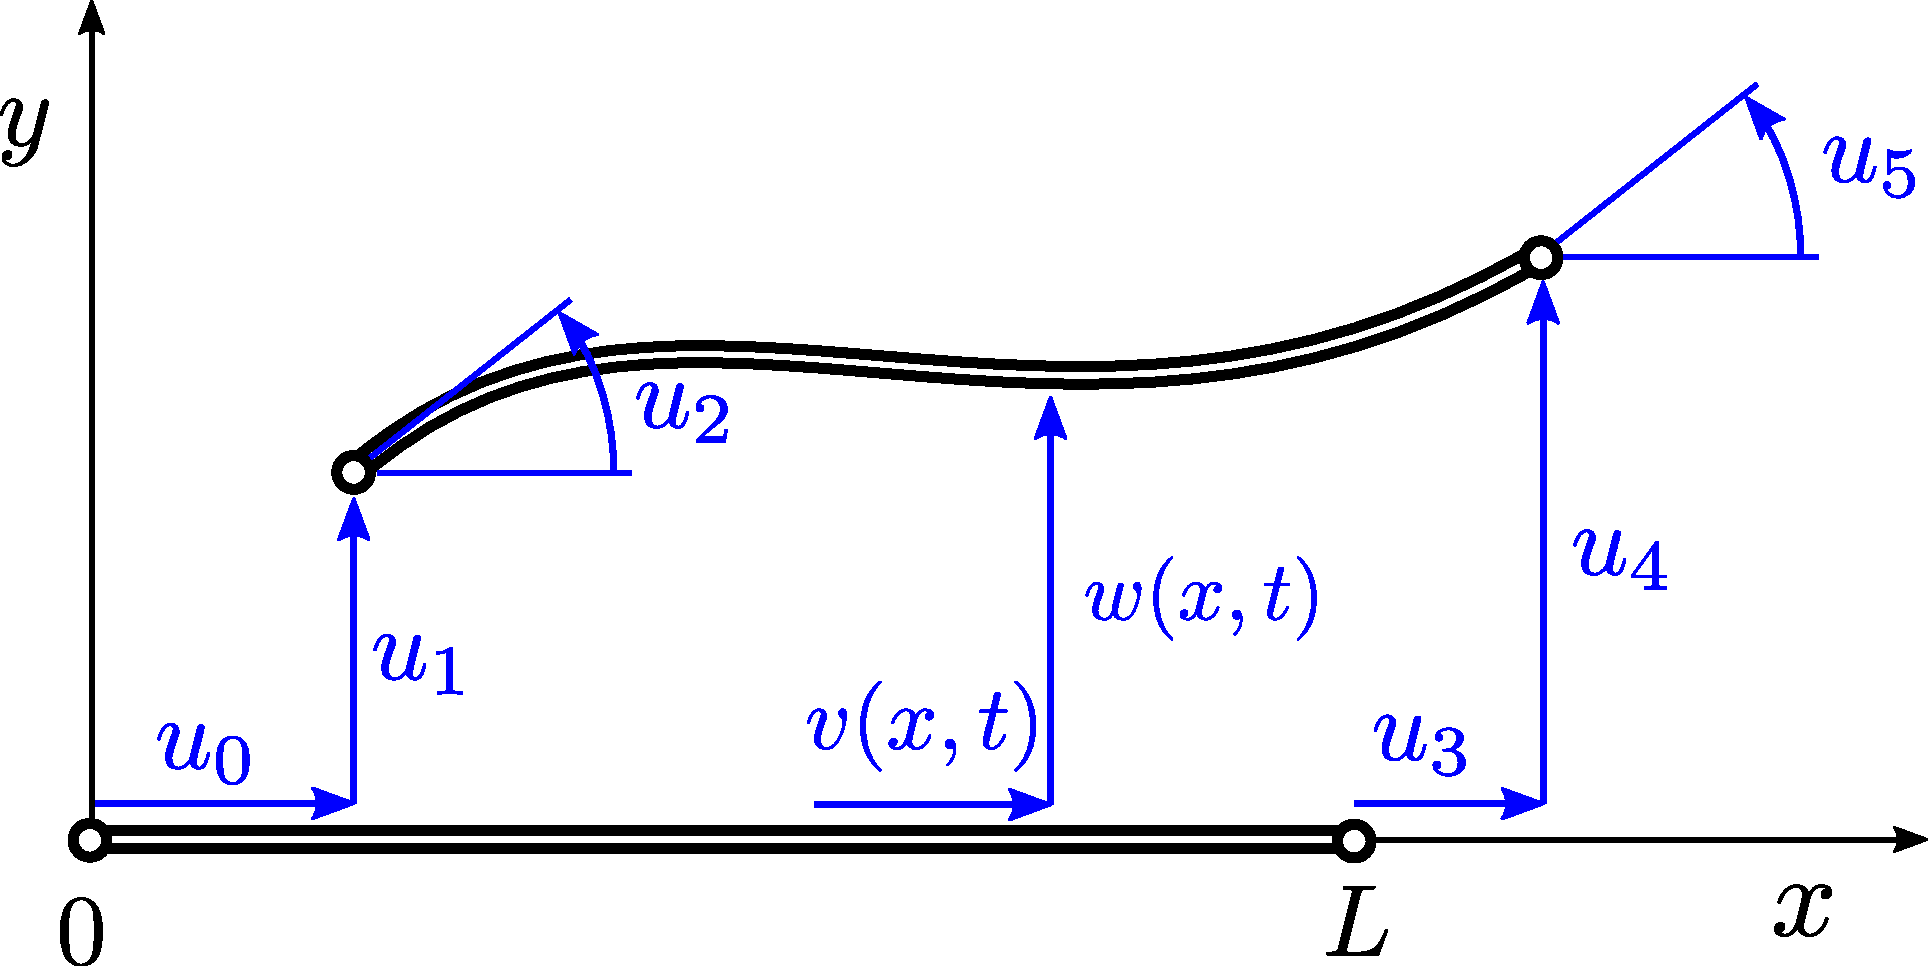
\includegraphics[width=0.7\textwidth]{figures/elements/beam-linear}
\caption{Beam element in reference and deformed configurations}
\label{fig:beam-linear}
\end{figure}

The finite element approach involves discretising this continuous displacement field by a finite number of degrees of freedom. This is achieved by choosing the nodal dispacements~$\boldsymbol{u}(t) = \begin{bmatrix}u_{0}(t),\ldots,\,u_{5}(t)\end{bmatrix}^\mathsf{T}$ as the degrees of freedom and interpolating~$v(x,t)$ and~$w(x,t)$ as

\begin{align}
v(x,t) &\approx \boldsymbol{V}(x)\,\boldsymbol{u}(t),\\
w(x,t) &\approx \boldsymbol{W}(x)\,\boldsymbol{u}(t),
\end{align}

with the shape functions~$\boldsymbol{V}(x)$ and~$\boldsymbol{W}(x)$.
As can be seen from figure~\ref{fig:beam-linear} the shape functions have to be chosen such that the following boundary conditions in regards to the nodal displacements are satisfied,

\begin{align}
v(0,t) &= u_{0}(t), & w(0,t) &= u_{1}(t), & w'(0,t) &= u_{2}(t),\notag\\
v(L,t) &= u_{3}(t), & w(L,t) &= u_{4}(t), & w'(L,t) &= u_{5}(t).\label{eq:elements:beam:boundary_conditions}
\end{align}

As the displacements were said to be small, the rotation angles of the nodes have been assumed to be equal to the derivative~$w'$ of the bending line here (small angle approximation).
Most frequently, for this standard type of beam element, cubic polynomials are used for~$\boldsymbol{W}(x)$ and a linear ones for~$\boldsymbol{V}(x)$. Coincidentally that is also the exact analytical solution for the static deformation of the beam. The free constants in those polynomials are determined by the boundary conditions~(\ref{eq:elements:beam:boundary_conditions}). The results are given by~\cite{bib:tm4} as

\begin{align}
\boldsymbol{W}(x) &=
\begin{bmatrix}
0\\
(1-\frac{x}{L})^2\,(1+2\,\frac{x}{L})\\
x\,(1-\frac{x}{L})^2\\
0\\
\frac{x^2}{L^2}\,(3-2\,\frac{x}{L})\\
-\frac{x^2}{L}\,(1-\frac{x}{L})
\end{bmatrix}^\mathrm{T},
&
\boldsymbol{V}(x) &=
\begin{bmatrix}
1-\frac{x}{L}\\
0\\
0\\
\frac{x}{L}\\
0\\
0
\end{bmatrix}^\mathrm{T}.
\end{align}

We now have a kinematic description of the beam element that has only a finite number of degrees of freedom. The vector of elastic forces $\boldsymbol{q}(\boldsymbol{u})$ for the system can be obtained by differentiating the system's total potential energy~\cite{bib:wiki-lagrange}, which in turn can be calculated by integrating the product of forces and deformations over the element length,

\begin{equation}
\boldsymbol{q}(\boldsymbol{u}) = \frac{\partial}{\partial \boldsymbol{u}}\,V(\boldsymbol{u}) = \frac{\partial}{\partial \boldsymbol{u}}\left(\frac{1}{2}\int_0^L
\begin{bmatrix}
N\\
M
\end{bmatrix}^\mathrm{T}
\begin{bmatrix}
\varepsilon\\
\kappa
\end{bmatrix}
\mathrm{d}x\right).\label{eq:beam-linear-energy-1}
\end{equation}

Here, $N$ and~$M$ are the normal force and the bending moment within the beam's cross sections, while $\varepsilon$ and $\kappa$ are the corresponding longitudinal strain and curvature of the beam's centerline. They are related to each other by the constitutive equation

\begin{equation}
\begin{bmatrix}
N\\
M
\end{bmatrix}
=
\begin{bmatrix}
C_{\varepsilon\varepsilon} & C_{\varepsilon\kappa}\\
C_{\varepsilon\kappa} & C_{\kappa\kappa}
\end{bmatrix}
\begin{bmatrix}
\varepsilon\\
\kappa
\end{bmatrix}.\label{eq:beam-constitutive}
\end{equation}

The constants $C_{\varepsilon\varepsilon}$, $C_{\kappa\kappa}$ and $C_{\varepsilon\kappa}$ are linear-elastic constants of the beam's cross section and will be determined later when we look at laminated beams. Combining the constitutive equation~(\ref{eq:beam-constitutive}) with~(\ref{eq:beam-linear-energy-1}), the elastic forces turn into

\begin{align}
\boldsymbol{q}(\boldsymbol{u}) &= \frac{\partial}{\partial \boldsymbol{u}}\left(\frac{1}{2}\int_0^L
\begin{bmatrix}
\varepsilon\\
\kappa
\end{bmatrix}^\mathrm{T}
\begin{bmatrix}
C_{\varepsilon\varepsilon} & C_{\varepsilon\kappa}\\
C_{\varepsilon\kappa} & C_{\kappa\kappa}
\end{bmatrix}
\begin{bmatrix}
\varepsilon\\
\kappa
\end{bmatrix}
\mathrm{d}x\right).\label{eq:elements:beam:total_energy_intermediate}
\end{align}

The strain~$\varepsilon$ and curvature~$\kappa$ for this beam can be calculated as

\begin{align}
\varepsilon(x,t) &= u'(x,t) = \boldsymbol{V}'(x)\,\boldsymbol{u}(t),\\
\kappa(x,t) &= w''(x,t) = \boldsymbol{W}''(x)\,\boldsymbol{u}(t).
\end{align}

Substituting these into equation~(\ref{eq:elements:beam:total_energy_intermediate}) finally leads to the following expression for the elastic forces,

\begin{align}
\boldsymbol{q}(\boldsymbol{u}) &= \frac{\partial}{\partial \boldsymbol{u}}\left(\frac{1}{2}\,\boldsymbol{u}^\mathrm{T}(t)
\underbrace{
\left(
\int_0^L
\begin{bmatrix}
\boldsymbol{V}'(x)\\
\boldsymbol{W}''(x)
\end{bmatrix}^\mathrm{T}
\begin{bmatrix}
C_{\varepsilon\varepsilon} & C_{\varepsilon\kappa}\\
C_{\varepsilon\kappa} & C_{\kappa\kappa}
\end{bmatrix}
\begin{bmatrix}
\boldsymbol{V}'(x)\\
\boldsymbol{W}''(x)
\end{bmatrix}
\mathrm{d}x
\right)
}_{\boldsymbol{C}}
\,\boldsymbol{u}(t)\right),\notag\\
&= \boldsymbol{C}\,\boldsymbol{u}(t).
\end{align}

The internal forces depend linearly on the displacements in a way that is determined by the stiffness matrix $\boldsymbol{C}$. Carrying out the integration yields

\begin{equation}
\boldsymbol{C} =
\begin{bmatrix}
\frac{1}{L}\,C_{\varepsilon\varepsilon} &
0 &
\frac{1}{L}\,C_{\varepsilon\kappa} &
-\frac{1}{L}\,C_{\varepsilon\varepsilon} &
0 &
-\frac{1}{L}\,C_{\varepsilon\kappa}\\ \\
0 &
\frac{12}{L^3}\,C_{\kappa\kappa} &
\frac{6}{L^2}\,C_{\kappa\kappa} &
0 &
-\frac{12}{L^3}\,C_{\kappa\kappa} &
\frac{6}{L^2}\,C_{\kappa\kappa}\\
\\
\frac{1}{L}\,C_{\varepsilon\kappa} &
\frac{6}{L^2}\,C_{\kappa\kappa} &
\frac{4}{L}\,C_{\kappa\kappa} &
-\frac{1}{L}\,C_{\varepsilon\kappa} &
-\frac{6}{L^2}\,C_{\kappa\kappa} &
\frac{2}{L}\,C_{\kappa\kappa}\\ \\
-\frac{1}{L}\,C_{\varepsilon\varepsilon} &
0 &
-\frac{1}{L}\,{C_{\varepsilon\kappa}} &
\frac{1}{L}\,C_{\varepsilon\varepsilon} &
0 &
\frac{1}{L}\,C_{\varepsilon\kappa}\\ \\
0 &
-\frac{12}{L^3}\,C_{\kappa\kappa} &
-\frac{6}{L^2}\,C_{\kappa\kappa} &
0 &
\frac{12}{L^3}\,C_{\kappa\kappa} &
-\frac{6}{L^2}\,C_{\kappa\kappa}\\ \\
-\frac{1}{L}\,C_{\varepsilon\kappa} &
\frac{6}{L^2}\,C_{\kappa\kappa} &
\frac{2}{L}\,C_{\kappa\kappa} &
\frac{1}{L}\,C_{\varepsilon\kappa} &
-\frac{6}{L^2}\,C_{\kappa\kappa} &
\frac{4}{L}\,C_{\kappa\kappa}
\end{bmatrix}.\label{eq:beam-linear-stiffness-matrix}
\end{equation}

The next step will be to determine the elastic constants $C_{\varepsilon\varepsilon}$, $C_{\kappa\kappa}$ and $C_{\varepsilon\kappa}$ for the kind of cross sections we're interested in.

\newpage
\subsection{Laminated Cross Sections}

The following derivations have been adapted from~\cite{bib:tm2} and~\cite{bib:wiki-sandwich}. Consider the laminated cross section shown in figure~\ref{fig:composite-sections-1}.
It is symmetric with respect to the~$y$-axis, bends/rotates around the~$z$-axis and consists of a number of rectangular layers. Each layer has its own density~$\rho_i$ and elastic modulus~$E_i$.
The geometry of the layers is given by their width~$w_i$, height~$h_i$ and center position~$y_i$.

\begin{figure}[h]
\centering
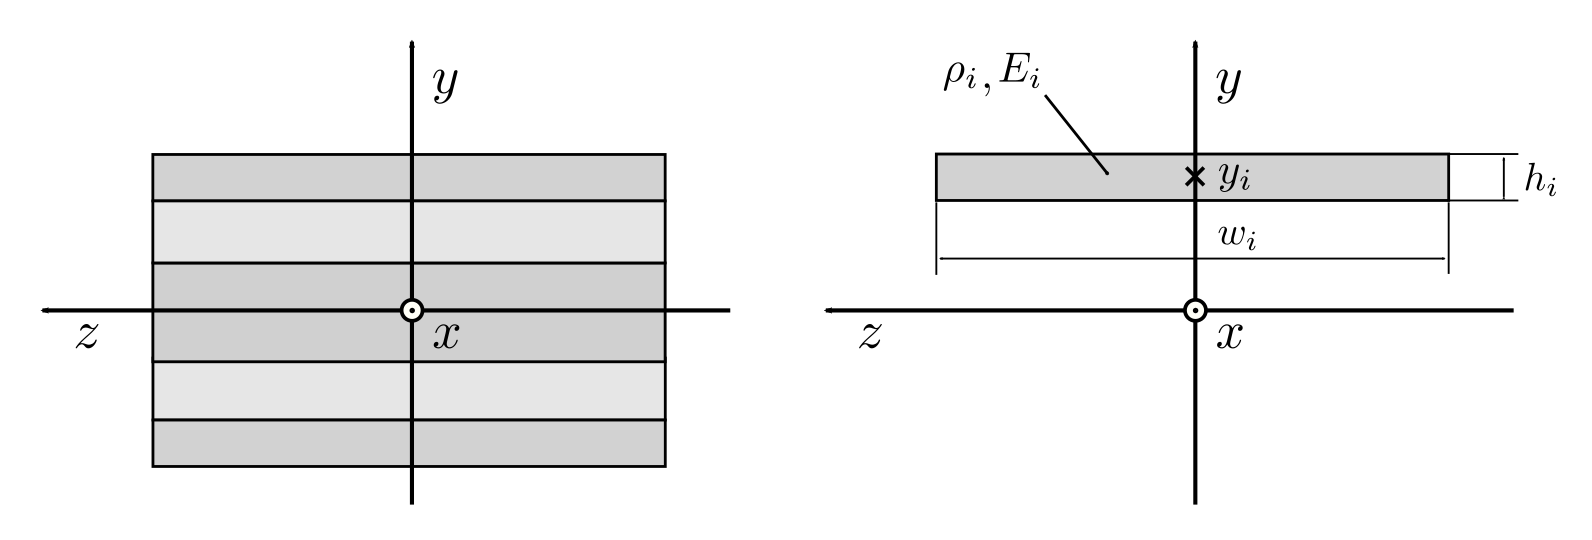
\includegraphics[width=0.9\textwidth]{figures/elements/composite-sections-1}
\caption{Composite cross section and single layer}
\label{fig:composite-sections-1}
\end{figure}

In Euler-Bernoulli beam theory the cross sections are assumed to stay flat and perpendicular to the beam axis during deformation.
We assume this to be true for our laminated cross section as well.
The distribution of longitudinal strain over the section is therefore given by the continuous function

\begin{equation}
\overline{\varepsilon}(y) = \varepsilon - \kappa\,y,
\end{equation}

where~$\varepsilon$ is the strain of the beam's centerline in $x$-direction and $\kappa$ its curvature around the $z$-axis.
The stress distribution however is not necessarily continuous, because each layer can have a different elastic modulus.
The stress within a layer is given by hooke's law as

\begin{equation}
\sigma_i(y) = E_i\cdot\overline{\varepsilon}(y),\quad y \in [y_i - \frac{h_i}{2},\,y_i + \frac{h_i}{2}].\label{eq:beam-stress-distribution}
\end{equation}

In order to determine the elastic constants in the constitutive equation~(\ref{eq:beam-constitutive}) we calculate the normal force~$N$ and bending moment~$M$ acting on the cross section by integrating the stresses~(\ref{eq:beam-stress-distribution}) over the section's area,

\begin{align}
N &= \int_A \sigma\,\mathrm{d}A = \sum_i\int_{A_i}\sigma_i\,\mathrm{d}A_i,\notag\\
&= \sum_i\int_{A_i}E_i\,\overline{\varepsilon}(y)\,\mathrm{d}A_i = \sum_i E_i \int_{A_i}(\varepsilon - \kappa\,y)\,\mathrm{d}A_i,\notag\\
&= \left(\sum_i E_i\int_{A_i}\mathrm{d}A_i\right)\varepsilon - \left(\sum_i E_i\int_{A_i}y\,\mathrm{d}A_i\right)\kappa,\notag\\
&=
\underbrace{
\left(\sum_i E_i\,A_i\right)
}_{C_{\varepsilon\varepsilon}}
\varepsilon
\underbrace{
- \left(\sum_i E_i\,A_i\,y_i\right)
}_{C_{\varepsilon\kappa}}
\kappa.\label{eq:elements:beam:constitutive_1}
\end{align}

The same can be done for the bending moment,

\begin{align}
M &= -\int_A y\,\sigma\,\mathrm{d}A = -\sum_i\int_{A_i}y\,\sigma_i\,\mathrm{d}A_i,\notag\\
&= -\sum_i\int_{A_i}y\,E_i\,(\varepsilon - \kappa\,y)\,\mathrm{d}A = -\sum_i\int_{A_i}(E_i\,\varepsilon\,y - E_i\,\kappa\,y^2)\,\mathrm{d}A,\notag\\
&= -\left(\sum_i E_i\int_{A_i}y\,dA_{i}\right)\varepsilon + \left(\sum_i E_i\int_{A_i}y^2\,dA_i\right)\kappa,\notag\\
&=
\underbrace{
-\left(\sum_i E_i\,A_i\,y_i\right)
}_{C_{\varepsilon\kappa}}
\varepsilon +
\underbrace{
\left(\sum_i E_i\,I_{i}\right)
}_{C_{\kappa\kappa}}
\kappa.\label{eq:elements:beam:constitutive_2}
\end{align}

The elastic constants describing the relationship between forces and deformation for the laminated cross section are therefore

\begin{align}
C_{\varepsilon\varepsilon} = \sum_i E_i\,A_i,\quad
C_{\kappa\kappa} = \sum_i E_i\,I_{i},\quad
C_{\varepsilon\kappa} = -\sum_i E_i\,A_i\,y_i.
\end{align}

In the case of the rectangular layers shown above, area~$A_i$ and second moment of inertia~$I_i$ evaluate to

\begin{align}
A_i &= w_i\,h_i,\\
I_i &= A_i\left(\frac{h_i^2}{12} + y_i^2\right).
\end{align}

Later we're also going to need the linear density (mass per unit length) of the laminated beam. It can be calculated by summing the the densities of the individual layers,

\begin{equation}
\overline{\rho A} = \sum_i \rho_i\,A_i.\label{eq:beam-linear-density}
\end{equation}

Pretty straightforward.

\newpage

\subsection{Floating Frame of Reference}

The floating frame of reference formulation is an easy way to construct a geometrically nonlinear finite element by reusing linear-elastic results.
The beam element is going to use a floating frame of reference approach based on~\cite{bib:beam_element_1} for the elastic forces, together with a lumped mass matrix according to~\cite{bib:beam_element_2}.
Key component is a floating frame of reference that is attached to the element and translates/rotates along with it.
The total motion of the element is then described as a superposition of two parts:

\begin{itemize}
\item The arbitrarily large, nonlinear rigid body motion (translation, rotation) of the reference frame
\item Small, linear-elastic deformations of the element with respect to its floating reference frame
\end{itemize}

Therefore the elastic deformation of the element can be treated as linear (because it's small), but on the other hand the element is still allowed to undergo arbitrarily large, nonlinear translations and rotations.
Note that we only assume the elastic deformations of the single elements to be small with respect to their frame of reference.
A structure composed of many such elements can still undergo large deformations as long as that assumption is valid. (And it can always be made valid by using enough elements.)

\begin{figure}[h]
\centering
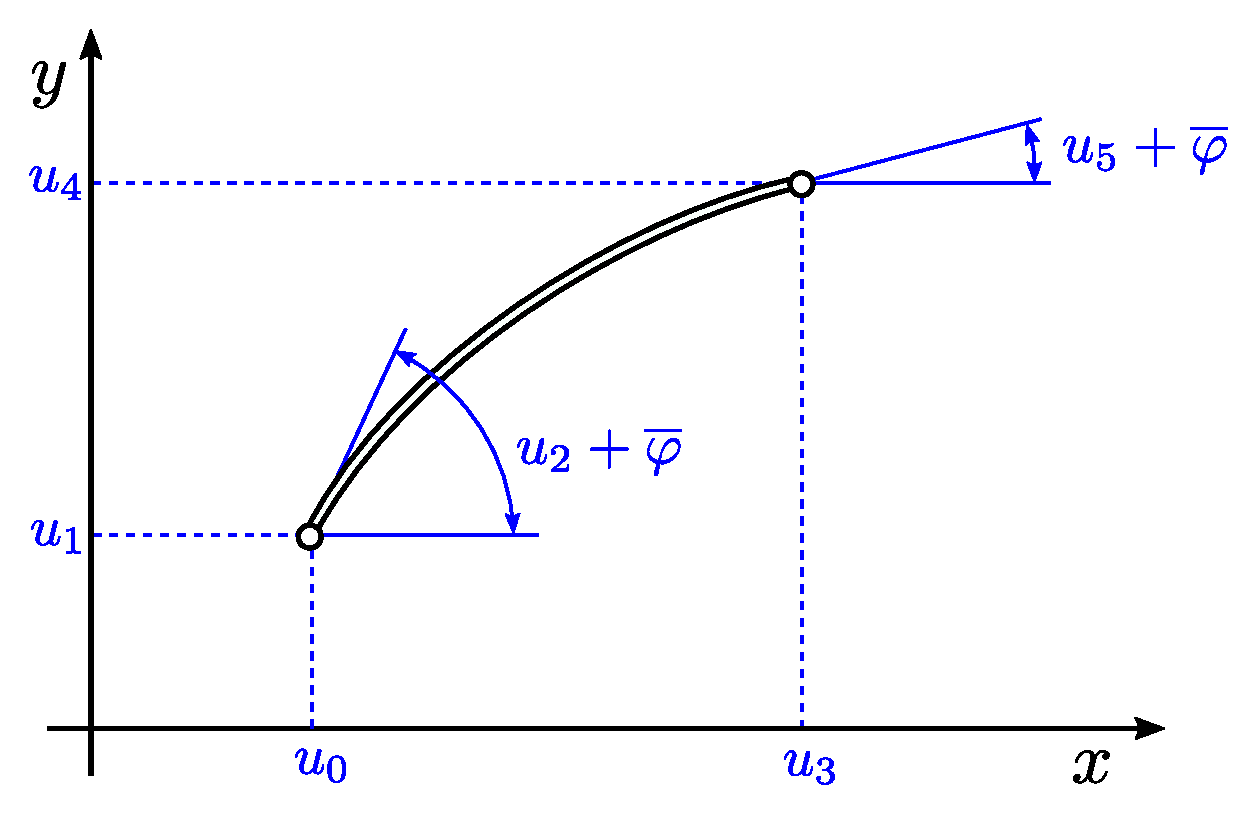
\includegraphics[width=0.6\textwidth]{figures/elements/beam-element-1}
\caption{Nodal displacements of the beam element}
\label{fig:beam-element-1}
\end{figure}

Let's apply this approach to the beam element shown in figure~\ref{fig:beam-element-1}. It has two nodes with the (arbitrarily large) nodal displacements~$\boldsymbol{u} = (u_0,\,\ldots,u_5)$ measured against the~$\{x,\,y\}$ coordinate system. The angle $\overline{\varphi}$ is a simple offset so that the rotation angles~$u_2$ and~$u_5$ don't necessarily have to correspond to the beam axis. This helps in practice when two adjacent elements share a node but are not tangential to each other.

We now introduce a floating frame of reference~$\{x',\,y'\}$ as shown in figure~\ref{fig:beam-element-2}. The $x'$-axis passes through both of the nodes (secant system) and the coordinate origin is placed at the left node. Within this reference system we now describe the elastic deformation with the three displacements~$\boldsymbol{e} = (e_0,\,e_1,\,e_2)^\mathsf{T}$, where~$e_0$ is the longitudinal extension of the beam and~$e_1$,~$e_2$ are the rotation angles of the nodes with respect to the~$x'$-axis.

\begin{figure}[h]
\centering
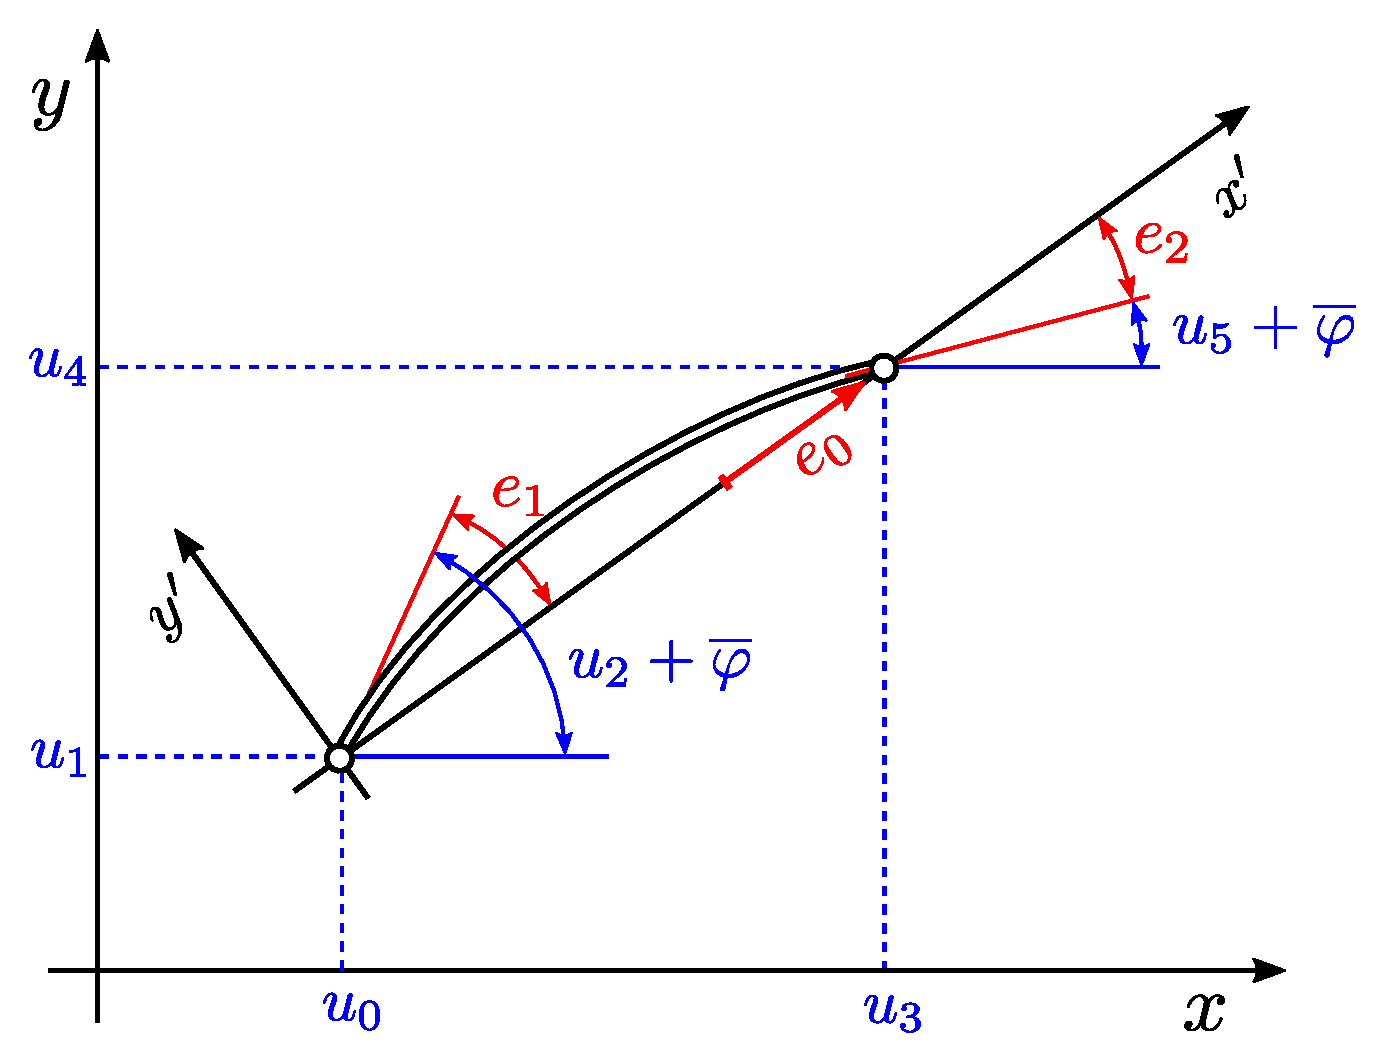
\includegraphics[width=0.6\textwidth]{figures/elements/beam-element-2}
\caption{Floating frame of reference and elastic deformations}
\label{fig:beam-element-2}
\end{figure}

Now obviously the elastic displacements~$\boldsymbol{e}$ depend on the overall displacements~$\boldsymbol{u}$ in some way, so the first thing we'll do is express this kinematic relationship. We introduce the auxiliary variables

\begin{align}
&\Delta x = u_3 - u_0,\\
&\Delta y = u_4 - u_1,\\
&\varphi = \mathrm{atan2} \left( \frac{\Delta y}{\Delta x} \right).
\end{align}

Here, $\varphi$ is the rotation angle of the floating reference frame. Using these abbreviations we can calculate the elastic deformations by using some elementary geometry.

\begin{align}
\intertext{Calculating $e_0$:}
&e_0 = \sqrt{\Delta x^2 + \Delta y^2} - L\\
\intertext{Calculating $e_1$:}
&\sin{(e_1)} = \sin{(u_2 + \overline{\varphi} - \varphi)} = \sin{(u_2)}\cos{(\overline{\varphi} - \varphi)} + \cos{(u_2)}\sin{(\overline{\varphi} - \varphi)}
\notag\\
&\cos{(e_1)} = \cos{(u_2 + \overline{\varphi} - \varphi)} = \cos{(u_2)}\cos{(\overline{\varphi} - \varphi)} - \sin{(u_2)}\sin{(\overline{\varphi} - \varphi)}\notag\\
&e_1 = \arctan{\left( \frac{\sin{(e_1)}}{\cos{(e_1)}} \right)}
\intertext{Calculating $e_2$:}
&\sin{(e_2)} = \sin{(u_5 + \overline{\varphi} - \varphi)} = \sin{(u_5)}\cos{(\overline{\varphi} - \varphi)} + \cos{(u_5)}\sin{(\overline{\varphi} - \varphi)}\notag\\
&\cos{(e_2)} = \cos{(u_5 + \overline{\varphi} - \varphi)} = \cos{(u_5)}\cos{(\overline{\varphi} - \varphi)} - \sin{(u_5)}\sin{(\overline{\varphi} - \varphi)}\notag\\
&e_2 = \arctan{\left( \frac{\sin{(e_2)}}{\cos{(e_2)}} \right)}
\intertext{Putting all those together, the elastic deformations can be written as}
&\boldsymbol{e}(\boldsymbol{u}) =
\begin{bmatrix}
\sqrt{\Delta x^2 + \Delta y^2} - L\\
\arctan{\left(\frac{\sin{(u_2)}\cos{(\overline{\varphi} - \varphi)}+\cos{(u_2)}\sin{(\overline{\varphi} - \varphi)}}{\cos{(u_2)}\cos{(\overline{\varphi} - \varphi)}-\sin{(u_2)}\sin{(\overline{\varphi} - \varphi)}}\right)}\\
\arctan{\left(\frac{\sin{(u_5)}\cos{(\overline{\varphi} - \varphi)}+\cos{(u_5)}\sin{(\overline{\varphi} - \varphi)}}{\cos{(u_5)}\cos{(\overline{\varphi} - \varphi)}-\sin{(u_5)}\sin{(\overline{\varphi} - \varphi)}}\right)}
\end{bmatrix}.\label{eq:beam-kinematics}
\end{align}

Having this out of the way, the vector of elastic forces~$\boldsymbol{q}(\boldsymbol{u})$ for the element will be obtained by differentiating the total potential energy~$V$ with respect to the displacements~$\boldsymbol{u}$,

\begin{equation}
\boldsymbol{q}(\boldsymbol{u}) = \frac{\partial V}{\partial \boldsymbol{u}}.\label{eq:beam-derivative}
\end{equation}

Now because we consider the beam as linear-elastic within its reference frame we can express its elastic energy as the quadratic expression

\begin{equation}
V = \boldsymbol{e}^\mathsf{T} \boldsymbol{C}\,\boldsymbol{e},
\end{equation}

where~$\boldsymbol{C}$ is the stiffness matrix of the beam. Its entries are a subset of the stiffness matrix ~(\ref{eq:beam-linear-stiffness-matrix}) that we derived earlier for the linear beam element,

\begin{equation}
\boldsymbol{C} =
\frac{1}{L}
\begin{bmatrix}
C_{\varepsilon\varepsilon} & -C_{\varepsilon\kappa} & C_{\varepsilon\kappa}\\
-C_{\varepsilon\kappa} & 4\,C_{\kappa\kappa} & 2\,C_{\kappa\kappa}\\
C_{\varepsilon\kappa} & 2\,C_{\kappa\kappa} & 4\,C_{\kappa\kappa}
\end{bmatrix}.
\end{equation}

Using this expression for the beam's energy, equation~(\ref{eq:beam-derivative}) becomes

\begin{align}
\boldsymbol{q}(\boldsymbol{u}) &= \frac{\partial V}{\partial \boldsymbol{u}} =  \frac{\partial V}{\partial \boldsymbol{e}}\,\frac{\partial \boldsymbol{e}}{\partial \boldsymbol{u}} = \left(\frac{\partial \boldsymbol{e}}{\partial \boldsymbol{u}}\right)^\mathsf{T}\boldsymbol{C}\,\boldsymbol{e}(\boldsymbol{u})\notag\\
&= \boldsymbol{J}(\boldsymbol{u})^\mathsf{T}\boldsymbol{C}\,\boldsymbol{e}(\boldsymbol{u}),
\end{align}

with the jacobian matrix $\boldsymbol{J}(\boldsymbol{u}) = \frac{\partial \boldsymbol{e}}{\partial \boldsymbol{u}}$. Differentiating~(\ref{eq:beam-kinematics}) gives us

\begin{align}
\boldsymbol{J}(\boldsymbol{u}) &= \frac{\partial \boldsymbol{e}}{\partial \boldsymbol{u}} =
\begin{bmatrix}
-J_{0} & -J_{1} & 0 & J_{0} & J_{1} & 0\\
-J_{3} & J_{2} & 1 & J_{3} & -J_{2} & 0\\
-J_{3} & J_{2} & 0 & J_{3} & -J_{2} & 1
\end{bmatrix},\\
\notag\\
J_{0} &= \frac{\Delta x}{\sqrt{\Delta x^2 + \Delta y^2}},\quad J_{1} = \frac{\Delta y}{\sqrt{\Delta x^2 + \Delta y^2}},\notag\\
\quad J_{2} &= \frac{\Delta x}{\Delta x^2 + \Delta y^2},\quad J_{3} = \frac{\Delta y}{\Delta x^2 + \Delta y^2}.
\end{align}

As always, the element's tangent stiffness matrix is obtained by differentiating the internal forces:

\begin{align}
\boldsymbol{K}(\boldsymbol{u}) &= \frac{\partial \boldsymbol{q}}{\partial \boldsymbol{u}} = \frac{\partial}{\partial \boldsymbol{u}}\left(\boldsymbol{J}^\mathsf{T}(\boldsymbol{u})\,\boldsymbol{C}\right)\boldsymbol{e}(\boldsymbol{u}) + \boldsymbol{J}^\mathsf{T}(\boldsymbol{u})\,\boldsymbol{C}\,\frac{\partial \boldsymbol{e}}{\partial \boldsymbol{u}}\notag\\
&= \left[\frac{\partial \boldsymbol{J}^\mathsf{T}(\boldsymbol{u})}{\partial u_{1}}\,\boldsymbol{C}\boldsymbol{e}(\boldsymbol{u}),\ldots \frac{\partial \boldsymbol{J}^\mathsf{T}(\boldsymbol{u})}{\partial u_{6}}\,\boldsymbol{C}\boldsymbol{e}(\boldsymbol{u})\right] + \boldsymbol{J}^\mathsf{T}(\boldsymbol{u})\,\boldsymbol{C}\,\boldsymbol{J}(\boldsymbol{u}).
\end{align}

The partial derivatives of the jacobian matrix~$\boldsymbol{J}$ are:

\begin{align}
\frac{\partial \boldsymbol{J}}{\partial u_0} &=
\begin{bmatrix}
-b_{0} & -b_{2} & 0 & b_{0} &  b_{2} & 0\\
-b_{5} &  b_{3} & 0 & b_{5} & -b_{3} & 0\\
-b_{5} &  b_{3} & 0 & b_{5} & -b_{3} & 0
\end{bmatrix},\quad
\frac{\partial \boldsymbol{J}}{\partial u_2} = 0,\quad
\frac{\partial \boldsymbol{J}}{\partial u_4} = -\frac{\partial \boldsymbol{J}}{\partial u_1},\notag\\
\frac{\partial \boldsymbol{J}}{\partial u_1} &=
\begin{bmatrix}
-b_{2} & -b_{1} & 0 & b_{2} &  b_{1} & 0\\
-b_{4} &  b_{5} & 0 & b_{4} & -b_{5} & 0\\
-b_{4} &  b_{5} & 0 & b_{4} & -b_{5} & 0
\end{bmatrix},\quad
\frac{\partial \boldsymbol{J}}{\partial u_3} = -\frac{\partial \boldsymbol{J}}{\partial u_0},\quad
\frac{\partial \boldsymbol{J}}{\partial u_5} = 0.
\end{align}

With the abbreviations

\begin{align}
a_{0} &= \frac{1}{(\Delta x^2 + \Delta y^2)^{\frac{1}{2}}},\quad
a_{1}  = \frac{1}{\Delta x^2 + \Delta y^2}\notag\\
a_{2} &= \frac{1}{(\Delta x^2 + \Delta y^2)^{\frac{3}{2}}},\quad
a_{3}  = \frac{1}{(\Delta x^2 + \Delta y^2)^{2}}\\
\notag\\
b_{0} &= a_{2}\Delta x^2 - a_{0},\quad b_{1} = a_{2}\Delta y^2 - a_{0},\quad b_{2} = a_{2}\Delta x\Delta y\notag\\
b_{3} &= 2a_{3}\Delta x^2 - a_{1},\quad b_{4} = 2a_{3}\Delta y^2 - a_{1},\quad b_{5} = 2a_{3}\Delta x\Delta y
\end{align}

The mass matrix is constructed by lumping the total mass and inertia of the element to the nodes, like before.
The total mass is~$\overline{\rho A}\,L$, using the linear density~(\ref{eq:beam-linear-density}) of the laminated cross sections.
Each translational degree of freedom therefore carries half of that mass. But the nodes also have a rotational degree of freedom each.
As it turns out, distributing the rotational inertia of a beam cannot be done in such a straightforward way.
There is simply no single "solution", only different approximations.
One possibility, according to~\cite{bib:beam_element_2}, is to use the mass matrix

\begin{equation}
\boldsymbol{M} = 
\overline{\rho A}\,L
\begin{bmatrix}
\frac{1}{2}\\
& \frac{1}{2}\\
&& \alpha L^2\\
&&& \frac{1}{2}\\
&&&& \frac{1}{2}\\
&&&&& \alpha L^2
\end{bmatrix},
\end{equation}

where~$\alpha \in\ ]0,\,\nicefrac{1}{50}]$ is a tunable parameter. Tests with the bow simulation suggest that the choice of~$\alpha$ barely has any influence on the results. Therefore the maximum value~$\alpha = \nicefrac{1}{50}$ has been chosen for numerical reasons.

\newpage
\subsection{Stiffness Matrix of a Beam Segment}

In this section the analytical stiffness matrix for a curved beam segment as shown in figure~\ref{fig:beam-linear-1} is derived following the approach presented in \cite{bib:curved-beam-stiffness-matrix}.

\begin{figure}[h]
\centering
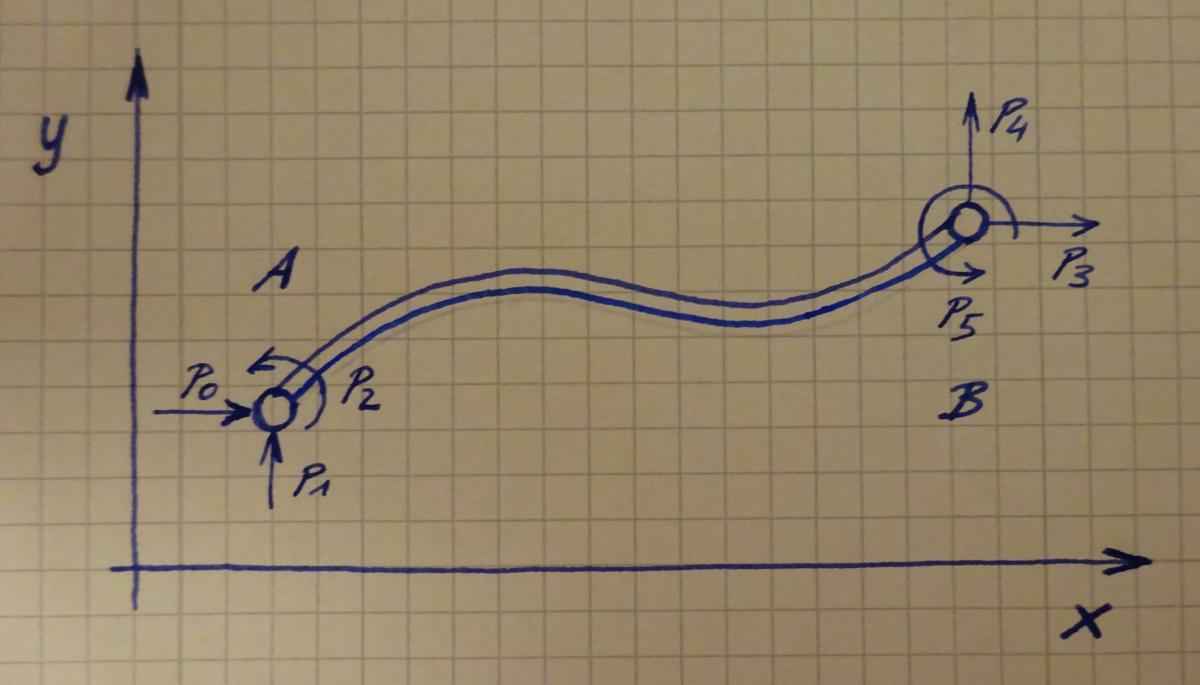
\includegraphics[width=0.5\textwidth]{figures/elements/beam-linear-1}
\caption{Curved beam segment with two nodes}
\label{fig:beam-linear-1}
\end{figure}

The segment has an initial length of~$l$. Its undeformed shape is described by the curve~$x(s)$, $y(s)$, $\varphi(s)$ with~$\varphi$ being the orientation angle measured against the $x$-axis and~$s \in [0,\,l]$ the arc length along the curve.

In order for the segment to be in static equilibrium, the nodal forces~$p_0$,\,\ldots\,$p_5$ have to fulfill the equilibrium conditions
%
\begin{align}
&p_0 + p_3 = 0 \\
&p_1 + p_4 = 0 \\
&p_2 + p_5 + p_0\,\Delta y - p1\,\Delta x = 0
\end{align}

where~$\Delta x = x(l) - x(0)$ and~$\Delta y = y(l) - y(0)$. This can be rearranged into the following matrix equation that relates the forces on nodes A and B to each other,

\begin{equation}
\underbrace{
\begin{bmatrix}
p_3 \\ p_4 \\ p_5
\end{bmatrix}
}_{\boldsymbol{p}_B}
=
\underbrace{
\begin{bmatrix}
-1 &  0 & 0 \\
 0 & -1 & 0 \\
-\Delta y & \Delta x & -1
\end{bmatrix}
}_{\boldsymbol{S}_{BA}}
\underbrace{
\begin{bmatrix}
p_0 \\ p_1 \\ p_2
\end{bmatrix}
}_{\boldsymbol{p}_A}
\label{eq:linear-beam-static-relation}
\end{equation}

\begin{figure}[h]
\centering
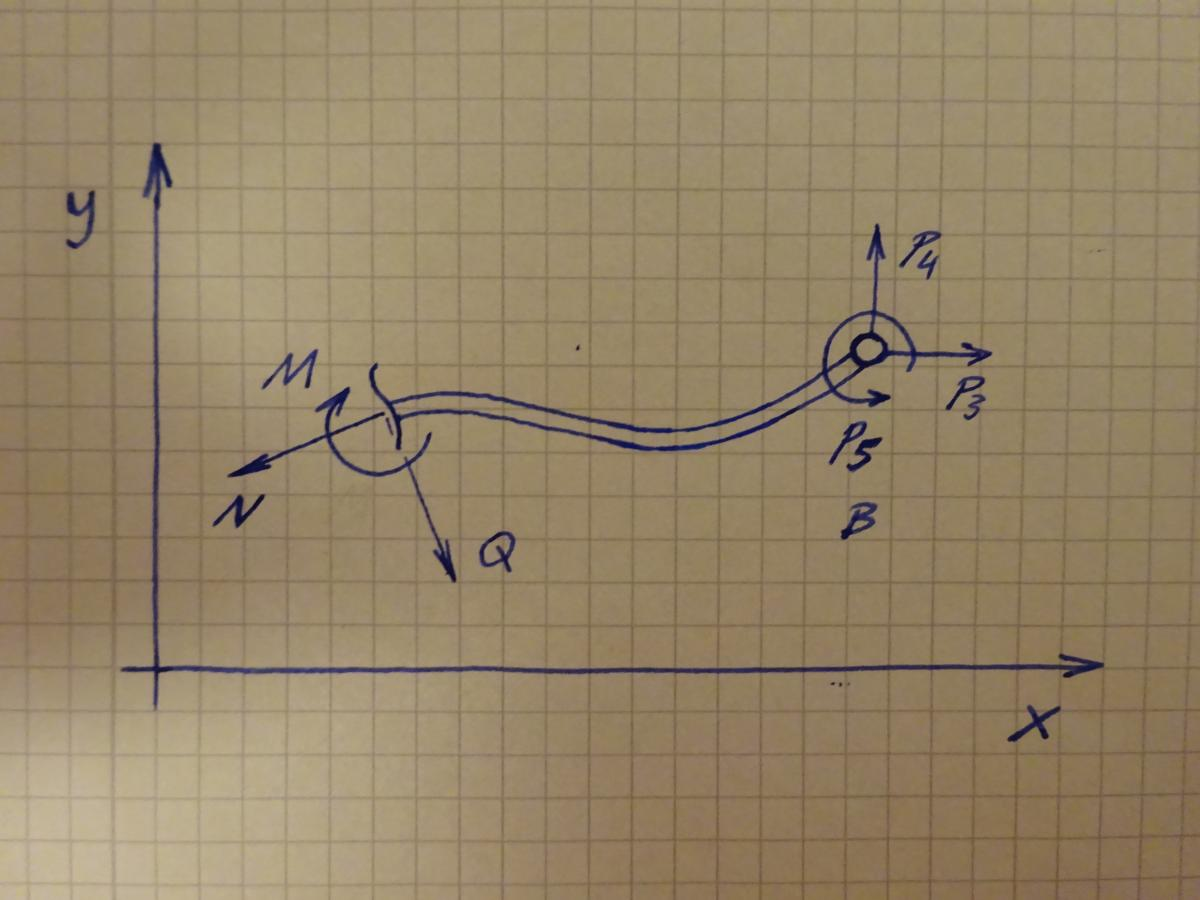
\includegraphics[width=0.5\textwidth]{figures/elements/beam-linear-2}
\caption{Cross section forces of the beam segment}
\label{fig:beam-linear-2}
\end{figure}

Forces on the cross section:

\begin{align*}
-&N(s)\cos(\varphi(s)) + Q(s)\sin(\varphi(s)) + p_3 = 0 \\
-&N(s)\sin(\varphi(s)) - Q(s)\cos(\varphi(s)) + p_4 = 0 \\
-&M(s) - p_3\,(y(l)-y(s)) + p_4\,(x(l) - x(s)) + p_5 = 0
\end{align*}

\begin{equation}
\begin{bmatrix}
N \\ M
\end{bmatrix}
=
\underbrace{
\begin{bmatrix}
\cos(\varphi(s)) & \sin(\varphi(s)) & 0 \\
y(s) - y(l) & x(l) - x(s) & 1
\end{bmatrix}
}_{\boldsymbol{H}_B(s)}
\underbrace{
\begin{bmatrix}
p_3 \\ p_4 \\ p_5
\end{bmatrix}
}_{\boldsymbol{p}_B}
\end{equation}


\subsubsection*{Case 1: Flexibility matrix of point B when A is fixed}

\begin{align}
V_B &= \frac{1}{2}\int_{0}^{l}
\begin{bmatrix}
N \\ M
\end{bmatrix}^\mathrm{T}
\begin{bmatrix}
\varepsilon \\ \kappa
\end{bmatrix}
ds \\
&= \frac{1}{2}\int_{0}^{l}
\begin{bmatrix}
N \\ M
\end{bmatrix}^\mathrm{T}
\begin{bmatrix}
C_{\varepsilon\varepsilon} & C_{\varepsilon\kappa}\\
C_{\varepsilon\kappa} & C_{\kappa\kappa}
\end{bmatrix}^{-1}
\begin{bmatrix}
N \\ M
\end{bmatrix}
ds \\
&= \frac{1}{2}\,\boldsymbol{p}_B^\mathrm{T}
\underbrace{
\left(\int_{0}^{l} \boldsymbol{H}_B^\mathrm{T}\,
\boldsymbol{C}^{-1}\boldsymbol{H}_B\,ds\right)
}_{\boldsymbol{K}_{BB}^{-1}}
\boldsymbol{p}_B
\end{align}

According to Castigliano's second theorem the displacement of node B under the external loads~$\boldsymbol{p}_B$ is

\begin{equation}
\boldsymbol{u}_{B} = \frac{\partial V_B}{\partial \boldsymbol{p}_B} = \boldsymbol{K}_{BB}^{-1}\,\boldsymbol{p}_B
\end{equation}

with the flexibility matrix~$\boldsymbol{K}_{BB}^{-1}$ which is the inverse of the stiffness matrix.

\subsubsection*{Case 2: Flexibility matrix of point A when B is fixed}

\begin{equation}
\begin{bmatrix}
N \\ M
\end{bmatrix}
= \boldsymbol{H}_B\,\boldsymbol{p}_B = \boldsymbol{H}_B\,\boldsymbol{S}_{BA}\,\boldsymbol{p}_A
\end{equation}

\begin{align}
V_A &= \frac{1}{2}\,\boldsymbol{p}_A^\mathrm{T}
\left(\int_{0}^{l} \boldsymbol{H}_A^\mathrm{T}\,
\boldsymbol{C}^{-1}\boldsymbol{H}_A\,ds\right)
\boldsymbol{p}_A \\
&= \frac{1}{2}\,\boldsymbol{p}_A^\mathrm{T}
\boldsymbol{S}_{BA}^\mathrm{T}\left(\int_{0}^{l} \boldsymbol{H}_B^\mathrm{T}\,
\boldsymbol{C}^{-1}\boldsymbol{H}_B\,ds\right)\boldsymbol{S}_{BA}\,\boldsymbol{p}_A \\
&= \frac{1}{2}\,\boldsymbol{p}_A^\mathrm{T}
\underbrace{
\left(\boldsymbol{S}_{BA}^\mathrm{T}\boldsymbol{K}_{BB}^{-1}\boldsymbol{S}_{BA}\right)
}_{\boldsymbol{K}_{AA}^{-1}}
\boldsymbol{p}_A 
\end{align}

Displacement of node A under the external loads~$\boldsymbol{p}_A$,

\begin{equation}
\boldsymbol{u}_{A} = \frac{\partial V_A}{\partial \boldsymbol{p}_A} = \boldsymbol{K}_{AA}^{-1}\,\boldsymbol{p}_A
\end{equation}

\subsubsection*{Non block-diagonal stiffness}

\begin{equation}
\boldsymbol{p}_B = \boldsymbol{S}_{BA}\,\boldsymbol{p}_A =
\underbrace{
\boldsymbol{S}_{BA}\,\boldsymbol{K}_{AA}
}_{\boldsymbol{K}_{BA}}
\,\boldsymbol{u}_A
\end{equation}

Therefore the complete stiffness relation for the beam segment is

\begin{equation}
\begin{bmatrix}
\boldsymbol{p}_A \\ \boldsymbol{p}_B
\end{bmatrix}
=
\begin{bmatrix}
\boldsymbol{K}_{AA} & \boldsymbol{K}_{BA}^\mathrm{T} \\
\boldsymbol{K}_{BA} & \boldsymbol{K}_{BB}
\end{bmatrix}
\begin{bmatrix}
\boldsymbol{u}_A \\ \boldsymbol{u}_B
\end{bmatrix}
\end{equation}

Note that this is an exact result. No simplifications have been made within the linear Euler-Bernoulli beam theory.





































\newpage
\section{Contact element}

The contact element is used to treat contact between a point and a surface. It uses a simple penalty approach: If the distance between the point and the surface is positive, there is no contact and nothing happens. But if the distance is negative, a contact force proportional to the penetration is applied that pushes the point outwards. By selecting a reasonably high contact stiffness the penetration can be kept small enough for all practical purposes.

\begin{figure}[h]
\centering
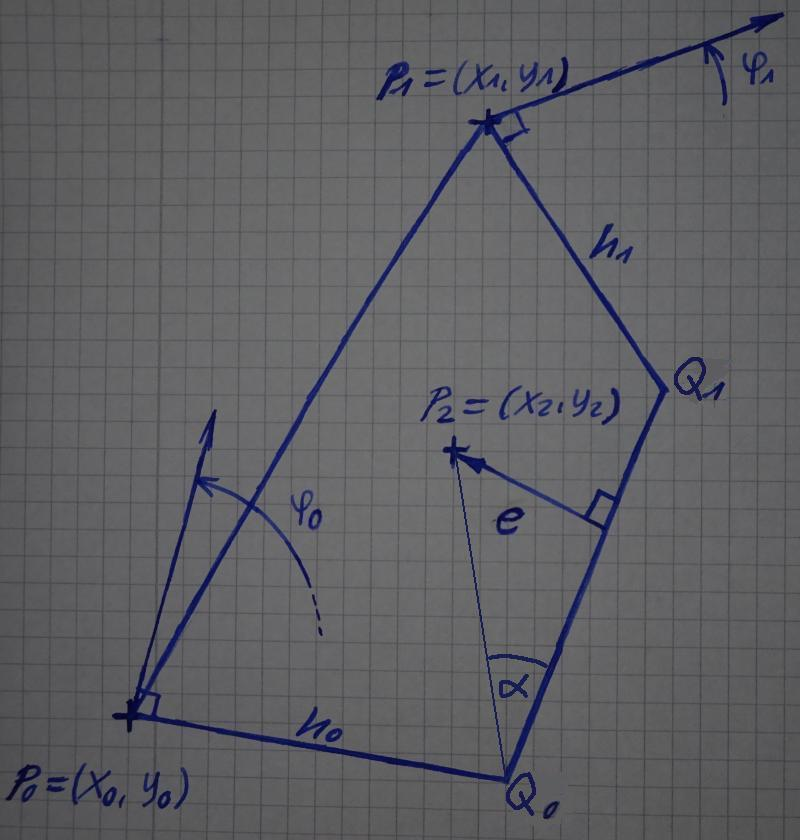
\includegraphics[width=0.5\textwidth]{figures/elements/contact_element_0}
\caption{Contact element}
%\label{fig:contact_element}
\end{figure}

\subsection{Contact Detection}

\textbf{Contact detection 1: Bounding box test}

\begin{align*}
x_{\rm{min}} &= \min\{x_0 - h_0,\:x_1 - h_1\}\\
y_{\rm{min}} &= \min\{y_0 - h_0,\:y_1 - h_1\}\\
x_{\rm{max}} &= \max\{x_0 + h_0,\:x_1 + h_1\}\\
y_{\rm{max}} &= \max\{y_0 + h_0,\:y_1 + h_1\}
\end{align*}

Necessary conditions for $P_2$ intersecting the segment:

\begin{align*}
x_{\rm{min}} \le x_{\rm{P2}} \le x_{\rm{max}}\\
y_{\rm{min}} \le y_{\rm{P2}} \le y_{\rm{max}}
\end{align*}

\textbf{Contact detection 2: Exact contact detection}

Coordinates of points $Q_0$ and $Q_1$:

\begin{equation*}
Q_0 = \begin{bmatrix}
x_{0} + h_{0}\sin(\varphi_{0}) \\
y_{0} - h_{0}\cos(\varphi_{0})
\end{bmatrix},\quad
Q_1 = \begin{bmatrix}
x_{1} + h_{1}\sin(\varphi_{1}) \\
y_{1} - h_{1}\cos(\varphi_{1})
\end{bmatrix}.
\end{equation*}

Define the four triangles

\begin{equation*}
T_{0} : \{ P_2, P_0, Q_0 \},\quad T_{1} : \{ P_2, P_1, P_0 \},\quad T_{2} : \{ P_2, Q_0, Q_1 \},\quad T_{3} : \{ P_2, Q_1, P_1 \}
\end{equation*}

$P_2$ lies inside the square if and only if all of the four triangles are oriented counter-clockwise. \textcolor{red}{[Citation needed]} % http://www.emanueleferonato.com/2012/03/09/algorithm-to-determine-if-a-point-is-inside-a-square-with-mathematics-no-hit-test-involved/
% https://en.wikipedia.org/wiki/Point_in_polygon

A triangle $\{A, B, C\}$ is oriented counter-clockwise if

\begin{align*}
&(B-A)\times(C-A) > 0,\\
\Leftrightarrow\quad &(x_B-x_A)(y_C-y_A)-(y_B-y_A)(x_C-x_A) > 0.
\end{align*}

\textbf{Contact detection 3: Penetration}

\begin{align*}
\sin(\alpha) &= \frac{e}{|P_2 - Q_0|} = \frac{(Q_1 - Q_0)\times(P_2 - Q_0)}{|Q_1 - Q_0||P_2 - Q_0|}\\
\\
\Leftrightarrow\:e &= \frac{(Q_1 - Q_0)\times(P_2 - Q_0)}{|Q_1 - Q_0|}\\
&= \frac{(x_{\rm{Q1}}-x_{\rm{Q0}})(y_{\rm{P2}}-y_{\rm{Q0}})-(y_{\rm{Q1}}-y_{\rm{Q0}})(x_{\rm{P2}}-x_{\rm{Q0}})}{\sqrt{(x_{\rm{Q1}}-x_{\rm{Q0}})^2+(y_{\rm{Q1}}-y_{\rm{Q0}})^2}}\\
&= \frac{a_1 a_4 - a_2 a_3}{\sqrt{a_1^2 + a_2^2}}
\intertext{With the abbreviations}
a_1 &= x_1 - x_0 - h_0 \sin(\varphi_0) + h_1 \sin(\varphi_1)\\
a_2 &= y_1 - y_0 + h_0 \cos(\varphi_0) - h_1 \cos(\varphi_1)\\
a_3 &= x_2 - x_0 - h_0 \sin(\varphi_0)\\
a_4 &= y_2 - y_0 + h_0 \cos(\varphi_0)
\end{align*}

\subsection{Contact Forces}

\textbf{Elastic forces}

The potential energy of the system can be determined as

\begin{align*}
V &= \int_{0}^{e}F(s)\,ds
\end{align*}

which yields the vector of elastic forces

\begin{align}
\boldsymbol{q}(\boldsymbol{u}) &= \frac{\partial V}{\partial \boldsymbol{u}} = \frac{\partial V}{\partial e}\frac{\partial e}{\partial \boldsymbol{u}} = F(e)\,\frac{\partial e}{\partial \boldsymbol{u}}.
\end{align}

Taking the derivatives:

\begin{align*}
\frac{\partial e}{\partial \boldsymbol{u}} &= \frac{\partial}{\partial \boldsymbol{u}}\left(\frac{a_1 a_4 - a_2 a_3}{\sqrt{a_1^2 + a_2^2}}\right)\\
&= \frac{\partial}{\partial \boldsymbol{u}}\left(\frac{1}{\sqrt{a_1^2 + a_2^2}}\right)\left(a_1 a_4 - a_2 a_3\right) + \frac{1}{\sqrt{a_1^2 + a_2^2}}\,\frac{\partial}{\partial \boldsymbol{u}}\left(a_1 a_4 - a_2 a_3\right)\\
&=
\underbrace{\frac{1}{\sqrt{a_1^2 + a_2^2}}}_{b_1} \underbrace{\left(a_4\frac{\partial a_1}{\partial \boldsymbol{u}} - a_3\frac{\partial a_2}{\partial \boldsymbol{u}} - a_2\frac{\partial a_3}{\partial \boldsymbol{u}} + a_1\frac{\partial a_4}{\partial \boldsymbol{u}}\right)}_{\boldsymbol{v}_1}
\underbrace{+\frac{a_2 a_3 - a_1 a_4}{(a_1^2 + a_2^2)^\frac{3}{2}}}_{b_2}
\underbrace{\left(a_1\frac{\partial a_1}{\partial \boldsymbol{u}} + a_2\frac{\partial a_2}{\partial \boldsymbol{u}}\right)}_{\boldsymbol{v}_2}\\
&= b_1\boldsymbol{v}_1 + b_2\boldsymbol{v}_2\\
\\
\frac{\partial a_1}{\partial \boldsymbol{u}} &=
\begin{bmatrix}
-1\\ 0\\ -h_0 \cos(\varphi_0)\\ 1\\ 0\\ h_1 \cos(\varphi_1)\\ 0\\ 0
\end{bmatrix},
\frac{\partial a_2}{\partial \boldsymbol{u}} =
\begin{bmatrix}
0\\ -1\\ -h_0 \sin(\varphi_0)\\ 0\\ 1\\ h_1 \sin(\varphi_1)\\ 0\\ 0
\end{bmatrix},
\frac{\partial a_3}{\partial \boldsymbol{u}} =
\begin{bmatrix}
-1\\ 0\\ -h_0 \cos(\varphi_0)\\ 0\\ 0\\ 0\\ 1\\ 0
\end{bmatrix},
\frac{\partial a_4}{\partial \boldsymbol{u}} =
\begin{bmatrix}
0\\ -1\\ -h_0 \sin(\varphi_0)\\ 0\\ 0\\ 0\\ 0\\ 1
\end{bmatrix}
\end{align*}

\textbf{Tangent stiffness matrix}

\begin{align*}
\boldsymbol{K}(\boldsymbol{u}) &= \frac{\partial \boldsymbol{q}}{\partial \boldsymbol{u}} = \frac{\partial F}{\partial \boldsymbol{u}}\,\left(\frac{\partial e}{\partial \boldsymbol{u}}\right)^{\rm{T}} + F(e)\,\frac{\partial^2 e}{\partial \boldsymbol{u}^2} = \frac{\partial F}{\partial e}\,\frac{\partial e}{\partial \boldsymbol{u}}\left(\frac{\partial e}{\partial \boldsymbol{u}}\right)^{\rm{T}} + F(e)\,\frac{\partial^2 e}{\partial \boldsymbol{u}^2}\\
\\
\frac{\partial^2 e}{\partial \boldsymbol{u}^2} &= \frac{\partial}{\partial \boldsymbol{u}}\left(b_1\boldsymbol{v}_1 + b_2\boldsymbol{v}_2\right) = \frac{\partial b_1}{\partial \boldsymbol{u}}\,\boldsymbol{v}_1^{\rm{T}} + \frac{\partial b_2}{\partial \boldsymbol{u}}\,\boldsymbol{v}_2^{\rm{T}} + b_1\,\frac{\partial \boldsymbol{v}_1}{\partial \boldsymbol{u}} + b_2\,\frac{\partial \boldsymbol{v}_2}{\partial \boldsymbol{u}}\\
\frac{\partial b_1}{\partial \boldsymbol{u}} &= -\frac{1}{\left(a_1^2 + a_2^2\right)^{\frac{3}{2}}}\left(a_1\,\frac{\partial a_1}{\partial \boldsymbol{u}} + a_2\,\frac{\partial a_2}{\partial \boldsymbol{u}}\right)\\
\frac{\partial b_2}{\partial \boldsymbol{u}} &= \frac{\sqrt{a_1^2 + a_2^2}}{a_1^6 + 3\,a_1^4\,a_2^2 + 3\,a_1^2\,a_2^4 + a_2^6}\bigg(\left(2\,a_1^2\,a_4 - a_2^2\,a_4 - 3\,a_1\,a_2\,a_3\right)\frac{\partial a_1}{\partial \boldsymbol{u}}\\
&+ \left(a_1^2\,a_3 - 2\,a_2^2\,a_3 + 3\,a_1\,a_2\,a_4\right)\frac{\partial a_2}{\partial \boldsymbol{u}} + \left(a_2^3 + a_1^2\,a_2\right)\frac{\partial a_3}{\partial \boldsymbol{u}} + \left(-a_1^3 - a_1\,a_2^2\right)\frac{\partial a_4}{\partial \boldsymbol{u}}\bigg)\\
\\
\frac{\partial \boldsymbol{v}_1}{\partial \boldsymbol{u}} &= \frac{\partial a_4}{\partial \boldsymbol{u}}\left(\frac{\partial a_1}{\partial \boldsymbol{u}}\right)^{\rm{T}} - \frac{\partial a_3}{\partial \boldsymbol{u}}\left(\frac{\partial a_2}{\partial \boldsymbol{u}}\right)^{\rm{T}} - \frac{\partial a_2}{\partial \boldsymbol{u}}\left(\frac{\partial a_3}{\partial \boldsymbol{u}}\right)^{\rm{T}} + \frac{\partial a_1}{\partial \boldsymbol{u}}\left(\frac{\partial a_4}{\partial \boldsymbol{u}}\right)^{\rm{T}}\\
&+ a_4\,\frac{\partial^2 a_1}{\partial \boldsymbol{u}^2} - a_3\,\frac{\partial^2 a_2}{\partial \boldsymbol{u}^2} - a_2\,\frac{\partial^2 a_3}{\partial \boldsymbol{u}^2} + a_1\,\frac{\partial^2 a_4}{\partial \boldsymbol{u}^2}\\
\frac{\partial \boldsymbol{v}_2}{\partial \boldsymbol{u}} &=  \frac{\partial a_1}{\partial \boldsymbol{u}}\left(\frac{\partial a_1}{\partial \boldsymbol{u}}\right)^{\rm{T}} + \frac{\partial a_2}{\partial \boldsymbol{u}}\left(\frac{\partial a_2}{\partial \boldsymbol{u}}\right)^{\rm{T}} + a_1\,\frac{\partial^2 a_1}{\partial \boldsymbol{u}^2} + a_2\,\frac{\partial^2 a_2}{\partial \boldsymbol{u}^2}
\end{align*}

Second derivatives:

\begin{equation*}
\begin{aligned}
\left(\frac{\partial^2 a_1}{\partial \boldsymbol{u}^2}\right)_{ij} &=
\begin{cases}
\:\:\:h_0\,\sin(\varphi_0) & \text{$ij = (3,3)$}\\
-h_1\,\sin(\varphi_1) & \text{$ij = (6,6)$}\\
\:\:\:0 & \text{otherwise}
\end{cases}\\
\left(\frac{\partial^2 a_3}{\partial \boldsymbol{u}^2}\right)_{ij} &=
\begin{cases}
\:\:\:h_0\,\sin(\varphi_0) & \text{$ij = (3,3)$}\\
\:\:\:0 & \text{otherwise}
\end{cases}\\
\end{aligned}
\qquad
\begin{aligned}
\left(\frac{\partial^2 a_2}{\partial \boldsymbol{u}^2}\right)_{ij} &=
\begin{cases}
-h_0\,\cos(\varphi_0) & \text{$ij = (3,3)$}\\
\:\:\:h_1\,\cos(\varphi_1) & \text{$ij = (6,6)$}\\
\:\:\:0 & \text{otherwise}
\end{cases}\\
\left(\frac{\partial^2 a_4}{\partial \boldsymbol{u}^2}\right)_{ij} &=
\begin{cases}
-h_0\,\cos(\varphi_0) & \text{$ij = (3,3)$}\\
\:\:\:0 & \text{otherwise}
\end{cases}
\end{aligned}
\end{equation*}

\subsection{Broadphase Algorithm}

\chapter{Solving the Equations of Motion}

\section{Static Solution}

\textcolor{red}{Static solution in context of bow: Bracing and equilibrium path, necessity for load control and displacement control}

A System with the equation of motion

\begin{align}
\boldsymbol{M}\,\ddot{\boldsymbol{u}} + \boldsymbol{q}(\boldsymbol{u},\,\dot{\boldsymbol{u}}) = \boldsymbol{p}
\end{align}

is in static equilibrium if~$\dot{\boldsymbol{u}},\,\ddot{\boldsymbol{u}} = \boldsymbol{0}$, leading to the static equilibrium condition

\begin{align}
\boldsymbol{q}(\boldsymbol{u},\,\boldsymbol{0}) = \boldsymbol{p}\label{eq:statics:equilibrium}
\end{align}

for the displacements $\boldsymbol{u}$ and the external loads $\boldsymbol{p}$.
This is a nonlinear system of equations and can be interpreted as the internal elastic forces~$\boldsymbol{q}$ being in balance with the external loads.

\subsection{The Basic Newton-Raphson Method}

Most frequently, when solving static problems, the external loads are given and the task is to calculate the corresponding equilibrium displacements.
Equation~(\ref{eq:statics:equilibrium}) is then a nonlinear system of equations in $\boldsymbol{u}$. Solving it can only be done numerically except for very simple examples.

An often used method for this kind of problem is the Newton-Raphson method. The basic idea behind it is to linearise the equilibrium equation~(\ref{eq:statics:equilibrium}) around a known displacement vector~$\boldsymbol{u}_i$ and solve the resulting linear equation to obtain an improved approximation~$\boldsymbol{u}_{i+1}$. Starting with an initial value~$\boldsymbol{u}_0$ the procedure is repeated until the solution is accurate enough by some convergence criterion.

Linearising of (\ref{eq:statics:equilibrium}) yields

\begin{align}
\boldsymbol{q}(\boldsymbol{u}_i) +
\underbrace{
\left(\frac{\partial \boldsymbol{q}}{\partial \boldsymbol{u}}\bigg \vert_{\boldsymbol{u}_i}\right)
}_{\boldsymbol{K}(\boldsymbol{u}_i)}
\underbrace{
(\boldsymbol{u}_{i+1} - \boldsymbol{u}_i)
}_{\Delta\boldsymbol{u}_i} &= \boldsymbol{p}
\end{align}

Solving for $\Delta\boldsymbol{u}_i$ leads to the iterative procedure

\begin{align}
\Delta\boldsymbol{u}_i &= \boldsymbol{K}^{-1}(\boldsymbol{u}_i)\left(\boldsymbol{p} - \boldsymbol{q}(\boldsymbol{u}_i)\right),\\
\boldsymbol{u}_{i+1} &= \boldsymbol{u}_i + \Delta\boldsymbol{u}_i.\label{eq:statics:newton_iteration}
\end{align}

In the implementation the tangent stiffness matrix is not actually inverted, because that's expensive and potentially inaccurate. Instead,~$\Delta\boldsymbol{u}_i$ is obtained by solving the equivalent linear system of equations using a decomposition of the stiffness matrix. The symmetry of the tangent stiffness can be used here. (It isn't necessarily positive definite though, like the stiffness matrices of linear mechanical systems.)

Convergence criteria are usually formulated in terms of change in displacement~$\Delta\boldsymbol{u}$, the residuum $\boldsymbol{p} - \boldsymbol{q}$ or their product $\Delta\boldsymbol{u}^\mathsf{T}(\boldsymbol{p}-\boldsymbol{q})$ (which has the dimension of an energy). We will use the energy criterion

\begin{equation*}
\Delta\boldsymbol{u}_{i}^\mathsf{T}(\boldsymbol{p}-\boldsymbol{q}(\boldsymbol{u}_i)) < \varepsilon
\end{equation*}

The basic Newton-Raphson method can be improved and extended in many ways, for example by combining it with a line search or by avoiding the calculation of the tangent stiffness matrix at every iteration (simplified Newton-Raphson method, BFGS method \textcolor{red}{[Source]}).

\subsection{Constrained Newton-Raphson method}

In the previous section the Newton-Raphson method was applied to the problem of calculating the equilibrium displacements of a system when all applied forces are known. This method is used in VirtualBow for finding the braced equilibrium state of the bow (see section \textcolor{red}{[Reference]}). However, when calculating the draw curve we don't actually know the draw forces, just the displacement of the string center. \textcolor{red}{Also: Load decrease.}

A solution to this is displacement control, where we prescribe a value for one of the displacement components and instead treat the corresponding external forces as a variable that is determined during solution.

The following derivation has been adapted from \cite{fem_script_uni_bochum}. Displacement control is a special case of a wider class of methods where the equilibrium equations are modified as
%
\begin{align}
\boldsymbol{q}(\boldsymbol{u}) - \lambda\,\boldsymbol{p} &= 0,\label{eq:equilibrium_dc}\\
c(\boldsymbol{u},\,\lambda) &= 0.\label{eq:constraint_dc}
\end{align}
%
Here the external forces are scaled by the unknown load factor $\lambda$. To compensate for this additional unknown, a scalar constraint~$c(\boldsymbol{u},\,\lambda) = 0$ on the displacements and the load parameter is introduced. Depending on the choice of constraint the method can be turned into load control, displacement control or other more sophisticated schemes like the arc-length method. We will carry out the derivation for the general case and specify the constraints later. This is also how these methods are implemented in VirtualBow: A general implementation for arbitrary constraints that is then specialized into load controlled and displacement controlled methods by providing the necessary constraints.

The system of nonlinear equations (\ref{eq:equilibrium_dc}), (\ref{eq:constraint_dc}) has to be solved for the displacements~$\boldsymbol{u}$ and the load parameter~$\lambda$. Like before, the Newton-Raphson method is used: The equations are linearised around a given approximation~$\{\boldsymbol{u}_i,\,\lambda_i\}$ and solved to obtain an improved approximiation~$\{\boldsymbol{u}_{i+1},\,\lambda_{i+1}\}$. This is repeated iteratively until displacements and load parameter satisfy the equilibrium equations~(\ref{eq:equilibrium_dc}) as well as the constraint equation~(\ref{eq:constraint_dc}) reasonably well as determined by some convergence criterion.

Carrying out the linearisation leads to the two equations
%
\begin{align}
\boldsymbol{q}(\boldsymbol{u}) - \lambda\,\boldsymbol{p}\:&\approx\:\boldsymbol{q}(\boldsymbol{u_{i}}) - \lambda_i\,\boldsymbol{p} + 
\underbrace{
\frac{\partial \boldsymbol{q}}{\partial \boldsymbol{u}}(\boldsymbol{u_{i}})
}_{\boldsymbol{K_{i}}}
\underbrace{
(\boldsymbol{u_{i+1}} - \boldsymbol{u_{i}})
}_{\Delta\boldsymbol{u_{i}}}
- \boldsymbol{p}
\underbrace{
\,(\lambda_{i+1} - \lambda_{i})
}_{\Delta \lambda_{i}}
\notag\\
&\approx\ \boldsymbol{q}(\boldsymbol{u_{i}}) - \lambda_i\,\boldsymbol{p} + \boldsymbol{K_{i}}\,\Delta\boldsymbol{u_{i}} - \boldsymbol{p}\,\Delta \lambda_{i}\label{eq:equilibrium_dc_lin}\\
\notag\\
c(\boldsymbol{u},\,\lambda) \ &\approx\ c(\boldsymbol{u_{i}},\,\lambda_{i}) + \frac{\partial c}{\partial \boldsymbol{u}}(\boldsymbol{u_{i}},\,\lambda_{i})(\boldsymbol{u_{i+1}} - \boldsymbol{u_{i}}) + \frac{\partial c}{\partial \lambda}(\boldsymbol{u_{i}},\,\lambda_{i})(\lambda_{i+1} - \lambda_{i})\notag\\
&\approx\ c(\boldsymbol{u_{i}},\,\lambda_{i}) + \frac{\partial c}{\partial \boldsymbol{u}}(\boldsymbol{u_{i}},\,\lambda_{i})\,\Delta\boldsymbol{u_{i}} + \frac{\partial c}{\partial \lambda}(\boldsymbol{u_{i}},\,\lambda_{i})\,\Delta \lambda_{i}\label{eq:constraints_dc_lin}
\end{align}

Equations~(\ref{eq:equilibrium_dc_lin}) and~(\ref{eq:constraints_dc_lin}) can written as the single linear system of equations
%
\begin{align}
\begin{bmatrix}
\boldsymbol{K_{i}} & -\boldsymbol{p}\\
\frac{\partial c}{\partial \boldsymbol{u}}(\boldsymbol{u_{i}},\,\lambda_{i}) & \frac{\partial c}{\partial \lambda}(\boldsymbol{u_{i}},\,\lambda_{i})
\end{bmatrix}
\begin{bmatrix}
\Delta\boldsymbol{u_{i}}\\
\Delta \lambda_{i}
\end{bmatrix}
=
\begin{bmatrix}
\lambda_i\,\boldsymbol{p} - \boldsymbol{q}(\boldsymbol{u_{i}})\\
-\boldsymbol{c}(\boldsymbol{u_{i}},\,f_{i})
\end{bmatrix}.\label{eq:total_dc_lin}
\end{align}
%
Solving this for the increments in displacement and load factor $\{\Delta\boldsymbol{u_{i}},\,\Delta \lambda_{i}\}$ allows us to calculate the next values as
%
\begin{align}
\boldsymbol{u_{i+1}} = \boldsymbol{u_{i}} + \Delta\boldsymbol{u_{i}}\\
\lambda_{i+1} = \lambda_{i} + \Delta \lambda_{i}.
\end{align}
%
However, directly solving~(\ref{eq:total_dc_lin}) is not  numerically efficient because the augmented stiffness matrix is no longer symmetric. A much better way to solve this is block elimination. We use the first row of~(\ref{eq:total_dc_lin}) to express~$\Delta\boldsymbol{u_{i}}$ as
%
\begin{align}
\Delta\boldsymbol{u_{i}} &= \boldsymbol{\alpha} + \boldsymbol{\beta}\,\Delta \lambda_{i}.\label{eq:auxiliary_disp_dc}
\end{align}
%
With the auxiliary vectors
%
\begin{align}
\boldsymbol{\alpha} &= \boldsymbol{K_{i}^{-1}}(\lambda_i\,\boldsymbol{p} - \boldsymbol{q}(\boldsymbol{u_{i}}))\label{eq:auxiliary_1}\\
\boldsymbol{\beta} &= \boldsymbol{K_{i}^{-1}}\,\boldsymbol{p}\label{eq:auxiliary_2}
\end{align}
%
These can be computed efficiently by exploiting the symmetry of the stiffness matrix $\boldsymbol{K_{i}}$.
%
To calculate $\Delta \lambda_i$, we substitute~(\ref{eq:auxiliary_disp_dc}) into the second row of~(\ref{eq:total_dc_lin}) which gives us
%
\begin{align}
&\frac{\partial c}{\partial \boldsymbol{u}}(\boldsymbol{u_{i}},\,\lambda_{i})\Delta\boldsymbol{u_{i}} + \frac{\partial c}{\partial \lambda}(\boldsymbol{u_{i}},\,\lambda_{i})\,\Delta \lambda_{i} = -c(\boldsymbol{u_{i}},\,\lambda_{i})\notag\\
&\frac{\partial c}{\partial \boldsymbol{u}}(\boldsymbol{u_{i}},\,\lambda_{i})(\boldsymbol{\alpha} + \boldsymbol{\beta}\,\Delta \lambda_{i}) + \frac{\partial c}{\partial \lambda}(\boldsymbol{u_{i}},\,\lambda_{i})\,\Delta \lambda_{i} = -c(\boldsymbol{u_{i}},\,\lambda_{i})\notag\\
&\ \ \vdots\notag\\
&\Delta \lambda_{i} = -\frac{c(\boldsymbol{u_{i}},\,\lambda_{i}) + \frac{\partial c}{\partial \boldsymbol{u}}(\boldsymbol{u_{i}},\,\lambda_{i})\,\boldsymbol{\alpha}}{\frac{\partial c}{\partial \boldsymbol{u}}(\boldsymbol{u_{i}},\,\lambda_{i})\,\boldsymbol{\beta} + \frac{\partial c}{\partial \lambda}(\boldsymbol{u_{i}},\,\lambda_{i})}.\label{eq:res_load_factor}
\end{align}

The Newton-Raphson iteration is now complete. To summarize: First, calculate $\boldsymbol{\alpha}$ and~$\boldsymbol{\beta}$ by solving~(\ref{eq:auxiliary_1}) and~(\ref{eq:auxiliary_2}). Then calculate the increment of the load parameter by using~(\ref{eq:res_load_factor}). The increment in displacements is then obtained by equation~(\ref{eq:auxiliary_disp_dc}).\\

\subsection{Constraints for load- and displacement control}

Finally, the constraint function and the parametrisation of the load vector have to be chosen. To get a displacement controlled method as initially stated we choose the constraint function as
%
\begin{align}
\boldsymbol{c}(\boldsymbol{u},\,\lambda) = u^{(k)} - \overline{u}
\end{align}
%
where~$u^k$ is the $k$-th component of the displacement vector that we want to control and $\overline{u}$ is the prescribed value for it. The partial derivatives are
%
\begin{align*}
\frac{\partial c}{\partial \boldsymbol{u}} &= \boldsymbol{e}_k,\quad
\frac{\partial c}{\partial \lambda} = 0,
\end{align*}
%
with $\boldsymbol{e}_k$ being the $k$-th unit vector. If a load controlled method is needed instead, the constraint becomes
%
\begin{align}
\boldsymbol{c}(\boldsymbol{u},\,\lambda) = \lambda - \overline{\lambda},
\end{align}
%
with the desired load factor $\overline{\lambda}$. Partial derivatives:
%
\begin{align*}
\frac{\partial c}{\partial \boldsymbol{u}} &= \boldsymbol{0},\quad
\frac{\partial c}{\partial \lambda} = 1,
\end{align*}

\subsection{Line search}

There is one last extension to the Newton-Raphson method that is needed for our purposes and that is line search. 

\textcolor{red}{Todo: Explain line search and why it helps with contact handling}

\newpage
\subsection{Finding the Braced Equilibrium State}

\textcolor{red}{Length of the string...}

\section{Dynamic Solution}

The equations of motion together with the initial displacements~$\boldsymbol{u}_0$ and velocities~$\boldsymbol{v}_0$ of the system form the second-order initial value problem

\begin{align}
\boldsymbol{M}\ddot{\boldsymbol{u}} &+ \boldsymbol{q}(\boldsymbol{u},\,\ddot{\boldsymbol{u}}) = \boldsymbol{p},\quad \boldsymbol{u}(0) = \boldsymbol{u}_0,\ \ddot{\boldsymbol{u}}(0) = \boldsymbol{v}_0.\label{eq:dynamics:system_equation}
\end{align}

for the displacements~$\boldsymbol{u}(t)$.

Numerical solution methods for initial value problems can be grouped into explicit and implicit ones.
Explicit methods use the current state of the system at time~$t$ to calculate the next state at~$t + \Delta t$.
Implicit methods instead find the next state by solving an equation that involves the current and the next state.
In the context of finite element analysis, implicit methods require equilibrium iterations at every time step involving the system's tangent stiffness matrix, while explicit methods only require simple vector operations.
Implicit methods therefore have a higher computational cost per step, but can make up for it by requiring less steps overall, as their better stability allows them to use much larger step sizes than explicit methods.

Explicit methods are easier to implement and are a good choice for small time scales, like impact and wave propagation problems.
They are most effective when the computation of the time steps is fast, so they work well with constant, diagonal (lumped) mass matrices and simple elements with low-order shape functions.

Implicit methods in contrast are well suited for larger time scales, where explicit algorithms would need too many steps.
Examples are structural response problems or numerically stiff systems, i.e. systems whose eigenfrequencies range from very small to very large.

VirtualBow currently uses the central difference method \cite{bib:dynamic_solution}, which is an explicit method often used in FEM.
Based on it's properties and the advantages of explicit methods it seems like a good choice.
However, implicit methods have not yet been tested with VirtualBow. The Newmark-beta method \textcolor{red}{Source} for example might be worth a try.

VirtualBow previously used the Runge-Kutta-Fehlberg-7-8 method provided by the \textcolor{red}{the odeint library}.
It performed worse than the central difference method, probably because of the high number of function evaluations carried out by an order~7/8 Runge-Kutta scheme.
The big advantage however was the timestep control based on error estimation, which meant that absolutely no user input regarding the timestep was necessary.

\subsection{The Central Difference Method}

The continuous solution $\boldsymbol{u}(t)$ is approximated by the discrete values~$\boldsymbol{u}_i = \boldsymbol{u}(t_{i})$ at the equidistant time steps~$t_i = i\cdot\Delta t$,\ \ $i \in \mathbb{N}$.
The acceleration~$\ddot{\boldsymbol{u}}_i$ can be approximated by a central difference quotient as

\begin{align}
\ddot{\boldsymbol{u}}_i &= \frac{\boldsymbol{u}_{i+1} - 2\,\boldsymbol{u}_{i} + \boldsymbol{u}_{i-1}}{\Delta t^2}\label{eq:dynamics:difference_acceleration}
\end{align}

Solving for~$\boldsymbol{u}_{i+1}$ and calculating the accelerations~$\ddot{\boldsymbol{u}}_{i}$ from the equation of motion~(\ref{eq:dynamics:system_equation}) leads to

\begin{align}
\boldsymbol{u}_{i+1} &= 2\,\boldsymbol{u}_{i} - \boldsymbol{u}_{i-1} + \Delta t^2\,\ddot{\boldsymbol{u}}_{i}\notag\\
&= 2\,\boldsymbol{u}_{i} - \boldsymbol{u}_{i-1} + \Delta t^2\,\boldsymbol{M}^{-1}(\boldsymbol{p}_i - \boldsymbol{q}_i).
\end{align}

This expression is already the core of the method, it allows the calculation of the next displacements~$\boldsymbol{u}_{i+1}$ from the current and previous system states.
It only involves cheap vector operations as the mass matrix is diagonal and doesn't have to be "actually" inverted.

Only the velocity is still missing. For this the central difference quotients of the displacements~$\boldsymbol{u}_{i+1}$,~$\boldsymbol{u}_{i}$ and~$\boldsymbol{u}_{i-1}$ are used to calculate the intermediate velocities

\begin{align}
\dot{\boldsymbol{u}}_{i+\frac{1}{2}} &= \frac{\boldsymbol{u}_{i+1} - \boldsymbol{u}_{i}}{\Delta t},\\
\dot{\boldsymbol{u}}_{i-\frac{1}{2}} &= \frac{\boldsymbol{u}_{i} - \boldsymbol{u}_{i-1}}{\Delta t}.
\end{align} 

The actual new velocity~$\dot{\boldsymbol{u}}_{i+1}$ is linearly extrapolated from those,

\begin{align}
\dot{\boldsymbol{u}}_{i+1} &= \dot{\boldsymbol{u}}_{i+\frac{1}{2}} + \frac{1}{2}\,\left(\dot{\boldsymbol{u}}_{i+\frac{1}{2}} - \dot{\boldsymbol{u}}_{i-\frac{1}{2}}\right),\notag\\
&= \frac{1}{\Delta t}\,\left(\frac{3}{2}\,\dot{\boldsymbol{u}}_{i+1} - 2\,\dot{\boldsymbol{u}}_{i} + \frac{1}{2}\,\dot{\boldsymbol{u}}_{i-1}\right).
\end{align}

This last step is actually a custom modification as far as I can tell.
All descriptions of the central difference method that I've seen end with the calculation of~$\dot{\boldsymbol{u}}_{i+\frac{1}{2}}$.

The initialisation of the procedure needs some special attention, as the method uses the previous displacements~$\boldsymbol{u}_{i-1}$ that don't exist yet at time~$t = 0$.
Instead,~$\boldsymbol{u}_{-1}$ is estimated by using finite difference approximations of the system's initial velocity and acceleration:

\begin{align}
\dot{\boldsymbol{u}}_0 &= \frac{\boldsymbol{u}_{1} - \boldsymbol{u}_{-1}}{2\,\Delta t},\\
\ddot{\boldsymbol{u}}_0 &= \frac{\boldsymbol{u}_{1} - 2\,\boldsymbol{u}_{0} + \boldsymbol{u}_{-1}}{\Delta t^2},\\
&\Rightarrow \boldsymbol{u}_{-1} = \boldsymbol{u}_{0} - \Delta t\,\dot{\boldsymbol{u}}_{0} + \frac{\Delta t^2}{2}\,\ddot{\boldsymbol{u}}_{0}.
\end{align}

A last but very important question is how to choose the timestep~$\Delta t$.
The timestep influences the computational effort, the accuracy of the solution but most importantly the stability of the algorithm.
A too large time step will lead to a solution that "explodes" numerically.
For linear, conservative mechanical systems of the form

\begin{align}
\boldsymbol{M}\ddot{\boldsymbol{u}} + \boldsymbol{K}\boldsymbol{u} = \boldsymbol{p}
\end{align}

the stability condition is

\begin{align}
\Delta t \le \frac{2}{\omega_{max}}\label{eq:timestep_bound}
\end{align}

where~$\omega_{max}$ is the maximum natural frequency \cite{bib:dynamic_solution} of the system.
Unfortunately there is no such analytical bound on~$\Delta t$ that guarantees stability for nonlinear systems.
A common thing to do is to linearise the system around the current configuration and apply (\ref{eq:timestep_bound}) anyway.
A safety factor~$0 < \beta < 1$ is introduced to account for the uncertainties and the timestep is set to

\begin{align}
\Delta t = \beta \frac{2}{\omega_{max}}.
\end{align}

This doesn't guarantee stability in a strict sense, but it's okay for practical purposes. A common choice is~$\beta = 0.9$ but VirtualBow uses a lower value for the sake of robustness. The frequency $\omega_{max}$ is sometimes estimated by using the bound

\begin{align}
\omega_{max} \le \max_{i}\,\{\omega_{max,\,i}\}
\end{align}

where $\omega_{max,\,i}$ is the maximum natural frequency of the respective finite element~$i$. But this leads to larger time steps than necessary and actually causes more implementation effort than just solving the generalised eigenvalue problem

\begin{align}
\left(\boldsymbol{M} - \omega^2\boldsymbol{K}\right)\boldsymbol{\bar{u}} = 0\label{eq:natural_frequencies}
\end{align}

which is what VirtualBow does.

\textcolor{red}{No damping here. For a version with damping see the LS-Dyna theoretical manual of 2006.}

\subsection{Stopping Criterion and Progress Estimation}

The dynamic simulation is carried out until some stopping criterion is satisfied.
This criterion has to be chosen such that the simulated time interval contains all the information needed by the users while also keeping it as short as possible.
It has to include the separation of the arrow from the string plus some additional time, because some things like e.g. the maximum force on the string tend to happen only after the arrow left the bow.
A related requirement on the stopping criterion is that it must allow estimating the simulation progress, so that it can be shown to the user.

The simplest solution would be to simulate until a fixed time is reached.
This makes the progress estimation very easy, but it also has some drawbacks.
It would require users to specify the simulation time, which can only be found by trial and error and might have to be adjusted for different bows.

The current approach is to simulate the time interval~$[0,\,\alpha\,T]$ where~$T$ is the time for the arrow to reach brace height and~$\alpha$ is an arbitrary positive factor.
The default value is~$\alpha = 1.5$. The simulation progress at time~$\overline{t}$ can now be written as

\begin{equation}
\rm{progress} = \frac{\overline{t}}{\alpha\,T}\cdot 100\%.
\end{equation}

But only formally, because~$T$ is not yet known as long as~$\overline{t} < T$, i.e. as long as the arrow has not yet actually reached brace height.
For this first part of the simulation~$T$ is estimated by using the current time $\overline{t}$, arrow position $\overline{u}$ and arrow velocity $\overline{v}$ and extrapolating to the time when the arrow will reach the braced position $u_T$.
Assuming constant velocity, which is a very crude approximation, we can extrapolate the arrow position as
\begin{equation}
u(t) = \bar{u} + \bar{v}(t - \bar{t}).\label{eq:solution:progress:ansatz}
\end{equation}

Now $T$ can be calculated from by using the condition~$u(T) = u_T$, with results in
\begin{equation}
T = \frac{u_T - \bar{u}}{\bar{v}} + \bar{t}.
\end{equation}

This approximation is far from exact, but it is good enough for progress estimation and gets better the closer the arrow is to the braced position.
After the arrow has reached the braced position, the actual value of $T$ is known and used for the rest of the simulation.

\newpage
\section{Model setup}

\subsection{Finding the damping parameters}

The damping parameter $\eta A$ of the string is determined analytically such that the damping ratio associated with the first (longitudinal) natural frequency matches the user supplied value. From Appendix \ref{chapter:viscoelastic-bar-vibrations} it follows that
%
\begin{equation}
\eta A = \frac{4L}{\pi}\,\sqrt{\rho A\,EA}\,\zeta
\end{equation}

in order for this to be true, where $L$ is half the total length of the string to match the boundary conditions used.

\subsection{Distributing string elements}

\begin{figure}[h]
\centering
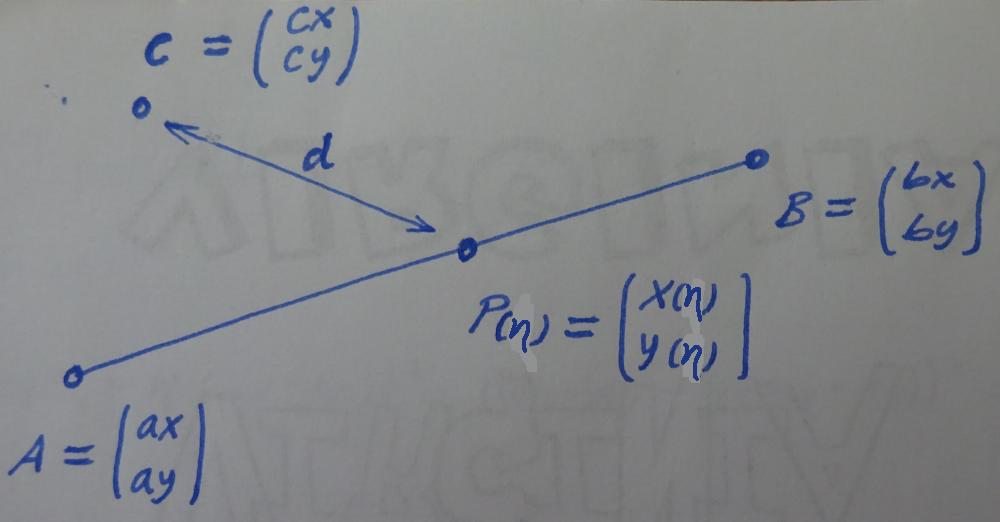
\includegraphics[width=0.8\textwidth]{figures/setup/line-distance}
\caption{Problem}
\label{fig:solution:dynamic_progress}
\end{figure}

Problem: Find a point $P$ on the line between $A$ and $B$ which has the euclidean distance $d$ to point $C$.

Parametrisation of the points $P$:

\begin{align*}
P(\eta) &= A + \eta\,(B-A),\quad \eta \in [0,\,1]
\end{align*}

Distance condition:

\begin{align*}
&\lVert C - P(\eta)\rVert = d\\
\Leftrightarrow\:&\lVert
\begin{bmatrix}
c_x - a_x - \eta\,(b_x - a_x) \\ c_y - a_y - \eta\,(b_y - a_y)
\end{bmatrix}
\rVert = d\\
\Leftrightarrow\:&\left(c_x - a_x - \eta\,(b_x - a_x)\right)^2 + \left(c_y - a_y - \eta\,(b_y - a_y)\right)^2 = d^2\\
\Leftrightarrow\:&\left((b_x - a_x)^2 + (b_y - a_y)^2\right)\,\eta^2-2\left((c_x - a_x)(b_x - a_x) + (c_y - a_y)(b_y - a_y)\right)\,\eta\\
&+(c_x - a_x)^2 + (c_y - a_y)^2 - d^2 = 0
\end{align*}

This is a quadratic equation for $\eta$. Take smallest solution in $[0,\,1]$.

\chapter{Model Validation} 

A very important task in the development of this software is to make sure that the results obtained by simulation agree reasonably well with real world examples.
This section shows the validation efforts made so far.
It is still very sparse, so if you have used this program for a real world application, let me know about your results and they will be added here.
\subsubsection{Statics of a straight steel bow}

In this experiment the draw curve and limb shapes of a small steel bow with a constant cross section have been measured and compared to version 2014.4 of Bow Simulation Tool (now \swtitle).
The bow is shown in figure~\ref{fig:validation:setup} and has been made from an old saw blade.
Steel is a good material for this kind of test because of its homogenous mechanical properties.
The elastic modulus was assumed to be $E = 210\ \rm{GPa}$ which is a good estimate for most types of steel.

\begin{figure}[H]
\centering
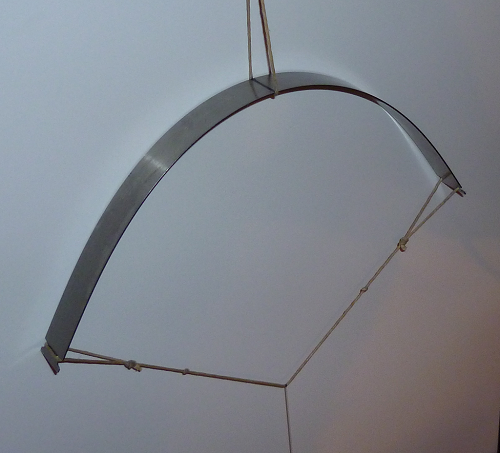
\includegraphics[width=0.5\textwidth]{figures/validation/setup.png}
\caption{Steel bow. Cross section:~16.85~$\times$~0.75mm. Length:~269mm. Brace heighth:~49.8mm}
\label{fig:validation:setup}
\end{figure}

The experiment was carried out by hanging a plastic bag at the string center.
The draw force was then gradually applied by counting steel balls with a known mass into the bag.
After every load step the draw length was measured and a photo of the bow was taken.

Figure~\ref{fig:validation:draw_curve} shows a comparison between the measured and the simulated draw curve and figure~\ref{fig:validation:limb_shapes} compares the pictures of the limb against the simulated limb shapes.

\begin{figure}[H]
\centering
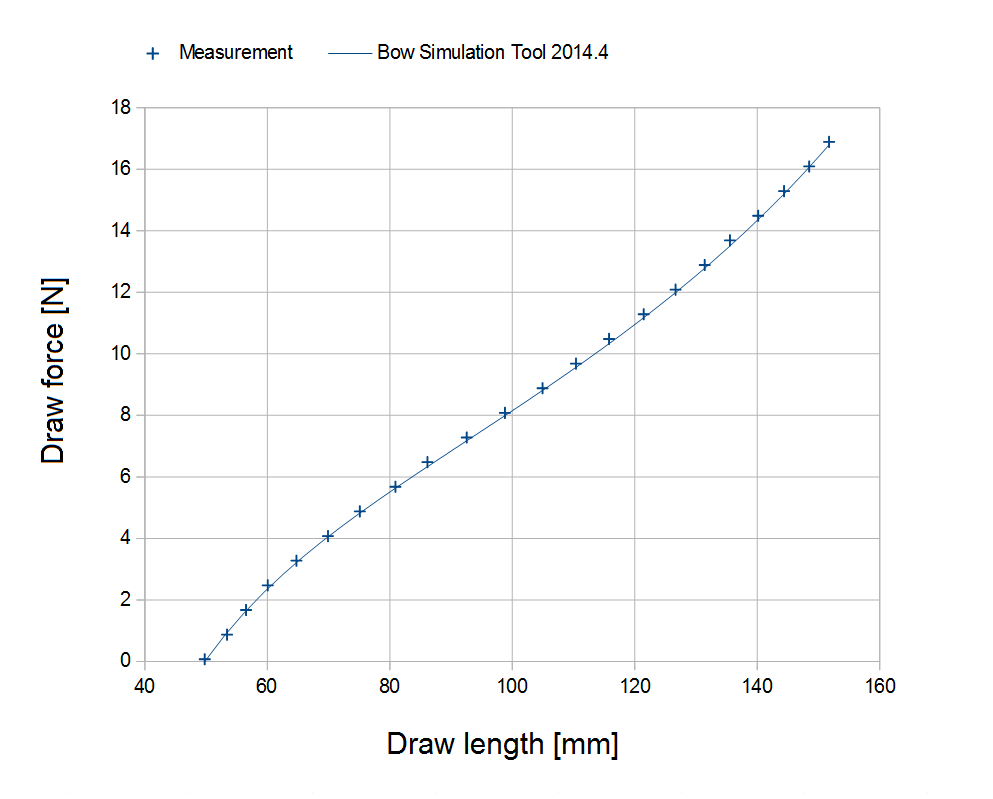
\includegraphics[width=0.85\textwidth]{figures/validation/draw_curve.png}
\caption{Experimental and simulated draw curves}
\label{fig:validation:draw_curve}
\end{figure}

\begin{figure}[H]
\centering
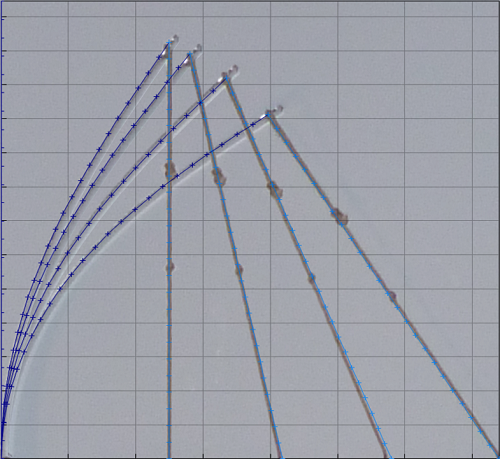
\includegraphics[width=0.65\textwidth]{figures/validation/states_blended.png}
\caption{Experimental and simulated limb shapes}
\label{fig:validation:limb_shapes}
\end{figure}

The agreement between experiment and simulation is surprisingly good here.
It really shows the potential of such kinds of simulations, provided that the material properties are well known and a the bow can be built exactly as simulated, with low tolerances.

But this is still a very simple example.
The next step would be to repeat this experiment with bows that have varying cross sections and non-straight profiles.
Another open question are the dynamic simulation results.
It's unclear if they can match experiments as good as the static results do, because there are much more uncertainties involved.

\appendix

\chapter{Vibrations of a viscoelastic bar}
\label{chapter:viscoelastic-bar-vibrations}

Consider the elastic bar shown in figure~\ref{fig:viscoelastic-bar}. It is fixed on the left hand side and free on the right, has a length of $L$ and can undergo longitudinal motion as described by the function $u(x,\,t)$. We want to calculate its (undamped) natural frequencies $\omega_0$ and associated damping ratios $\zeta$.

\begin{figure}[h]
\centering
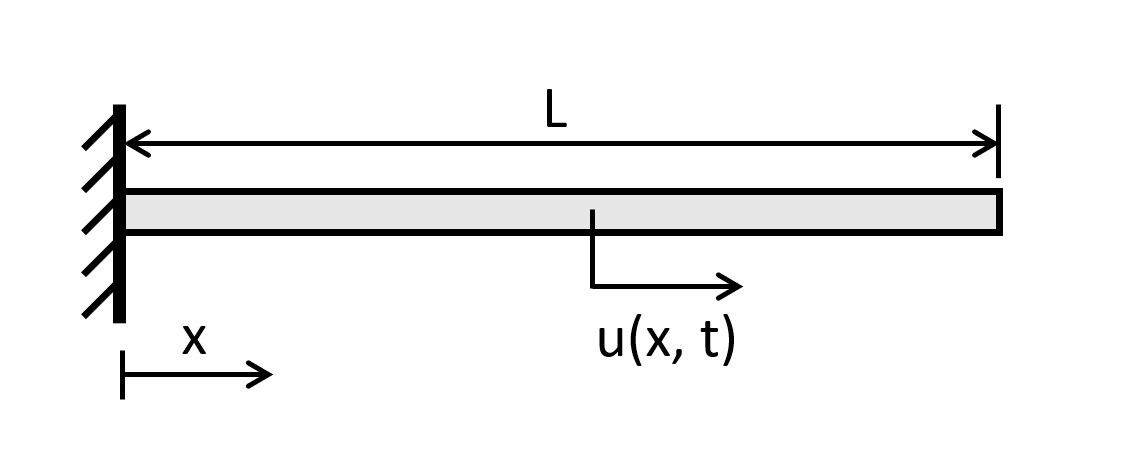
\includegraphics[width=0.5\textwidth]{figures/appendix/viscoelastic-bar}
\caption{Kinematics and boundary conditions of the bar}
\label{fig:viscoelastic-bar}
\end{figure}

The material of the bar is assumed to behave according to the viscoelastic Kelvin-Voigt model, which expresses the stress $\sigma$ in the bar as
%
\begin{equation}
\sigma = E\,\varepsilon + \eta\,\dot{\varepsilon}\label{eq:viscoelastic-bar-material}
\end{equation}

where $\varepsilon = \frac{\partial\,u}{\partial\,x}$ is the longitudinal strain, $E$ the elastic modulus and $\eta$ the viscosity of the material. The acceleration at every point in the bar is given by \textcolor{red}{Source?}
%
\begin{equation}
\rho\,\frac{\partial^2\,u}{\partial\,t^2} = \frac{\partial\,\sigma}{\partial\,x}\label{eq:viscoelastic-bar-kinetic}
\end{equation}

where $\rho$ is the bar's density. Combining the equations (\ref{eq:viscoelastic-bar-material}) and (\ref{eq:viscoelastic-bar-kinetic}) and multiplying with the cross section area $A$ results in the equation of motion
%
\begin{equation}
\rho A\,\frac{\partial^2\,u}{\partial\,t^2} = EA\,\frac{\partial^2\,u}{\partial\,x^2} + \eta A\,\frac{\partial^3\,u}{\partial\,x^2\,\partial\,t}.\label{eq:viscoelastic-bar-motion}
\end{equation}

This partial differential equation can be solved by separation of variables. The solution is assumed as $u(x,\,t) = X(x)\,T(t)$, a product of two functions depending on $x$ and $t$ respectively. Inserting this into the equation of motion (\ref{eq:viscoelastic-bar-motion}) and separating terms depending on $x$ from terms depending on $t$ leads to
%
\begin{align}
\rho A\,X(x)\,\ddot{T}(t) &= EA\,X''(x)\,T(t) + \eta A\,X''(x)\,\dot{T}(t)\notag \\
\frac{X''(x)}{X(x)} &= \frac{\ddot{T}(t)}{\frac{EA}{\rho A}\,T(t) + \frac{\eta A}{\rho A}\,\dot{T}(t)} =: -\frac{\rho A}{EA}\,\omega_0^2\label{eq:viscoelastic-bar-separated}
\end{align}

Apply the usual argument: As one side of the equation depends on position and the other on time they have to be constant in order to be equal. We choose that constant to be $-\frac{\rho A}{EA}\,\omega_0^2$ and obtain the two ordinary differential equations
%
\begin{align}
\ddot{T}(t) + \frac{\eta A}{EA}\,\omega_0^2\,\dot{T}(t) + \omega_0^2\,T(t) = 0,\label{eq:viscoelastic-bar-t} \\
X''(x) + \frac{\rho A}{EA}\,\omega_0^2\,X(x) = 0.\label{eq:viscoelastic-bar-x}
\end{align}

The time equation (\ref{eq:viscoelastic-bar-t}) describes a damped harmonic oscillator with undamped natural frequency $\omega_0$ and damping ratio
%
\begin{equation}
\zeta = \frac{1}{2}\,\frac{\eta\,A}{EA}\,\omega_0\label{eq:viscoelastic-bar-result-zeta}
\end{equation}

as determined by the coefficients of the equation. The last remaining task is to determine the natural frequencies $\omega_0$ which solve the second differential equation (\ref{eq:viscoelastic-bar-x}) while also satisfying the boundary conditions of the bar. The general solution of (\ref{eq:viscoelastic-bar-x}) is
%
\begin{equation}
X(x) = C\cdot\sin\left(\sqrt{\frac{\rho A}{EA}}\,\omega_0\,x - \varphi\right).
\end{equation}

Boundary condition on the fixed end:
%
\begin{align}
u(0,\,t) = 0: \quad\quad\quad X(0)\,T(t) &= 0 \notag \\
C\cdot\sin(-\varphi) &= 0 \notag \\
\varphi &= 0
\end{align}

The case $T(t) = 0$ was ignored here because it is of no interest. The boundary condition for the free end is
%
\begin{align}
\sigma(L,\,t) = 0: \quad\quad E\,\varepsilon(L,\,t) + \eta\,\dot{\varepsilon}(L,\,t) &= 0 \notag \\
EA\,\frac{\partial u}{\partial x}(L,\,t) + \eta A\,\frac{\partial^2 u}{\partial x\,\partial t}(L,\,t) &= 0 \notag \\
EA\,X'(L)\,T(t) + \eta A\,X'(L)\,\dot{T}(t) &= 0 \notag \\
(EA\,T(t) + \eta A\,\dot{T}(t))\,X'(L) &= 0 \notag \\
\ddot{T}(t)\,X'(L) &= 0 \notag
\end{align}

And therefore the solution for the natural frequencies is
%
\begin{align}
X'(L) &= C\cdot\sqrt{\frac{\rho A}{EA}}\,\omega_0\cos\left(\sqrt{\frac{\rho A}{EA}}\,\omega_0\,L\right) = 0, \notag \\
\omega_0 &= \frac{\pi(2k - 1)}{2L}\cdot\sqrt{\frac{EA}{\rho A}},\quad k \in \mathbb{Z}.\label{eq:viscoelastic-bar-result-omega}
\end{align}

And finally, with equations (\ref{eq:viscoelastic-bar-result-zeta}) and (\ref{eq:viscoelastic-bar-result-omega}) the damping ratio follow as
%
\begin{equation}
\zeta = \frac{\pi(2k - 1)}{4L}\cdot\frac{\eta A}{\sqrt{\rho A \cdot EA}},\quad k \in \mathbb{Z}.
\end{equation}

\chapter{Cubic Spline Interpolation}

Cubic splines are used to define some of the geometric features of the bow, namely the profile curve, width and layer heights.

\section{Cubic $C^2$ Spline}

Consider $n$ points $(x_{0},\,y_{0}) \ldots (x_{n-1},\,y_{n-1})$ with increasing values of $x$.
We define the differences $\Delta x_{i} = x_{i+1} - x_{i}$ and $\Delta y_{i} = y_{i+1} - y_{i}$ as well as the slope $\delta_{i} = \Delta y_{i} / \Delta x_{i}$ of the secant line between two successive points.

For each interval $x \in [x_{i},\,x_{i+1}]$ the data is interpolated by the cubic polynomial
%
\begin{align}
f_{i}(x) &= h_{00}(t)\,y_{i} + h_{10}(t)\Delta x_{i}\,m_{i} + h_{01}(t)\,y_{i+1} + h_{11}(t)\Delta x_{i}\,m_{i+1} \\
f_{i}'(x) &= \frac{h_{00}'(t)}{\Delta x_{i}}\,y_{i} + h_{10}'(t)\,m_{i} + \frac{h_{01}'(t)}{\Delta x_{i}}\,y_{i+1} + h_{11}'(t)\,m_{i+1} \\
f_{i}''(x) &= \frac{h_{00}''(t)}{\Delta x_{i}^2}\,y_{i} + \frac{h_{10}''(t)}{\Delta x_{i}}\,m_{i} + \frac{h_{01}''(t)}{\Delta x_{i}^2}\,y_{i+1} + \frac{h_{11}''(t)}{\Delta x_{i}}\,m_{i+1}
\end{align}
%
where $y_{i}$, $y_{i+1}$ and $m_{i}$, $m_{i+1}$ are the values and slopes at the interval boundaries, respectively and $h_{00}(t)\,\ldots\,h_{11}(t)$ are the hermite basis functions, defined as
%
\begin{equation}
\begin{aligned}
h_{00}(t) &= 2\,t^3 - 3\,t^2 + 1 \\
h_{10}(t) &= t^3 - 2\,t^2 + t \\
h_{01}(t) &= -2\,t^3 + 3\,t^2 \\
h_{11}(t) &= t^3 - t^2
\end{aligned}
\quad
\begin{aligned}
h_{00}'(t) &= 6\,t^2 - 6\,t \\
h_{10}'(t) &= 3\,t^2 - 4\,t + 1 \\
h_{01}'(t) &= -6\,t^2 + 6\,t \\
h_{11}'(t) &= 3\,t^2 - 2\,t
\end{aligned}
\quad
\begin{aligned}
h_{00}''(t) &= 12\,t - 6 \\
h_{10}''(t) &= 6\,t - 4 \\
h_{01}''(t) &= -12\,t + 6 \\
h_{11}''(t) &= 6\,t - 2
\end{aligned}
\end{equation}
%
with $t = (x - x_{i})/(x_{i+1} - x_{i})$. The resulting spline by definition already interpolates the given function values and is $C^1$ continuous since adjacent segments share the same value and slope at the interval boundaries.
To determine the $n$ unknown slopes $m_{i}$ we require the second derivatives at the connection points to match as well, making the curve $C^2$ continuous. This gives us $n-2$ continuity conditions, leaving two more conditions to make the problem uniquely determined.
Those additional conditions are obtained from boundary considerations, e.g. by specifying the spline's first and/or second derivatives at the left and right endpoints.

%https://math.stackexchange.com/questions/62360/natural-cubic-splines-vs-piecewise-hermite-splines

Continuity conditions $f_{i-1}''(x_{i}) = f_{i}''(x_{i})$ for $i = 1 \ldots n-2$:
%
\begin{align}
&\frac{h_{00}''(1)}{\Delta x_{i-1}^2}\,y_{i-1} + \frac{h_{10}''(1)}{\Delta x_{i-1}}\,m_{i-1} + \frac{h_{01}''(1)}{\Delta x_{i-1}^2}\,y_{i} + \frac{h_{11}''(1)}{\Delta x_{i-1}}\,m_{i} = \frac{h_{00}''(0)}{\Delta x_{i}^2}\,y_{i} + \frac{h_{10}''(0)}{\Delta x_{i}}\,m_{i} + \frac{h_{01}''(0)}{\Delta x_{i}^2}\,y_{i+1} + \frac{h_{11}''(0)}{\Delta x_{i}}\,m_{i+1} \notag \\
&\frac{-2}{\Delta x_{i}}\,m_{i+1} + \left(\frac{-4}{\Delta x_{i}} - \frac{4}{\Delta x_{i-1}}\right)\,m_{i} - \frac{2}{\Delta x_{i-1}}\,m_{i-1} = \frac{6\,y_{i-1} + -6\,y_{i}}{\Delta x_{i-1}^2} - \frac{-6\,y_{i} + 6\,y_{i+1}}{\Delta x_{i}^2} \notag \\
&\frac{1}{\Delta x_{i}}\,m_{i+1} + 2\left(\frac{1}{\Delta x_{i}} + \frac{1}{\Delta x_{i-1}}\right)\,m_{i} + \frac{1}{\Delta x_{i-1}}\,m_{i-1} = 3\left(\frac{\Delta\,y_{i}}{\Delta x_{i}^2} + \frac{\Delta y_{i-1}}{\Delta x_{i-1}^2}\right) \notag \\
&\Delta x_{i-1}\,m_{i+1} + 2\left(\Delta x_{i} + \Delta x_{i-1}\right)\,m_{i} + \Delta x_{i}\,m_{i-1} = 3\left(\delta_{i}\,\Delta x_{i-1} + \delta_{i-1}\,\Delta x_{i}\right)
\end{align}

Boundary condition $f_{0}''(0) = y_{0}''$:

\begin{align}
\frac{h_{00}''(0)}{\Delta x_{0}^2}\,y_{0} + \frac{h_{10}''(0)}{\Delta x_{0}}\,m_{0} + \frac{h_{01}''(0)}{\Delta x_{0}^2}\,y_{1} + \frac{h_{11}''(0)}{\Delta x_{0}}\,m_{1} = y_{0}''& \notag \\
\frac{-6}{\Delta x_{0}^2}\,y_{0} + \frac{-4}{\Delta x_{0}}\,m_{0} + \frac{6}{\Delta x_{0}^2}\,y_{1} + \frac{-2}{\Delta x_{0}}\,m_{1} = y_{0}''& \notag \\
4\,m_{0} + 2\,m_{1} = 6\,\delta_{0} - \Delta x_{0}\,y_{0}''&
\end{align}

Boundary condition $f_{n-2}''(1) = y_{n-1}''$:

\begin{align}
\frac{h_{00}''(1)}{\Delta x_{n-2}^2}\,y_{n-2} + \frac{h_{10}''(1)}{\Delta x_{n-2}}\,m_{n-2} + \frac{h_{01}''(1)}{\Delta x_{n-2}^2}\,y_{n-1} + \frac{h_{11}''(1)}{\Delta x_{n-2}}\,m_{n-1} = y_{n-1}''& \notag \\
\frac{6}{\Delta x_{n-2}^2}\,y_{n-2} + \frac{2}{\Delta x_{n-2}}\,m_{n-2} + \frac{-6}{\Delta x_{n-2}^2}\,y_{n-1} + \frac{4}{\Delta x_{n-2}}\,m_{n-1} = y_{n-1}''& \notag \\
2\,m_{n-2} + 4\,m_{n-1} = 6\,\delta_{n-2} + \Delta x_{n-2}\,y_{n-1}''&
\end{align}

Boundary condition $f_{0}'(0) = y_{0}'$:
%
\begin{equation}
m_{0} = y_{0}'
\end{equation}

Boundary condition $f_{n-1}'(1) = y_{n-1}'$:
%
\begin{equation}
m_{n-1} = y_{n-1}'
\end{equation}

Combining the continuity and boundary conditions gives us the system of equations
%
\begin{equation}
\begin{bmatrix}
a_{0} & b_{0} \\
& \ddots & \ddots & \ddots \\
&& \Delta x_{i-1} & 2(\Delta x_{i} + \Delta x_{i-1}) & \Delta x_{i} \\
&&& \ddots & \ddots & \ddots \\
&&&& a_{n-1} & b_{n-1}
\end{bmatrix}
\begin{bmatrix}
m_{0} \\
\vdots \\
m_{i} \\
\vdots \\
m_{n-1} \\
\end{bmatrix}
=
\begin{bmatrix}
c_{0} \\
\vdots \\
3\left(\delta_{i}\,\Delta x_{i-1} + \delta_{i-1}\,\Delta x_{i}\right) \\
\vdots \\
c_{n-1} \\
\end{bmatrix}
\end{equation}

where $a$, $b$ and $c$ depend on the choice of boundary conditions. Since the coefficient matrix has a tridiagonal structure it can be solved very efficiently by using the Thomas algorithm.

\section{Monotonicity}

Sometimes it is desirable for an interpolating curve to preserve monotonicity of the input data, i.e. not to introduce any local minima or maxima between the given data points.
In VirtualBow this is used for the width and layer heights, not least to ensure that those quantities are always positive if the user entered positive values.

One popular method for monotonic cubic interpolation is the Fritsch–Carlson method\cite{bib:fc80}, which operates on a cubic hermite spline like the one we defined above and adjusts the slopes according to some simple rules in order to make the spline monotonic within each interval.
The only difference is that Fritsch and Carlson use finite differences to determine the initial slopes for their spline while we used the condition of $C^2$ continuity.

After the initial slopes were computed, the first necessary condition for monotonicity in an interval is
%
\begin{equation}
\mathrm{sgn}(m_{i}) = \mathrm{sgn}(m_{i+1}) = \mathrm{sgn}(\delta_{i})
\end{equation}
%
which means that the slopes $m_{i}$ and $m_{i+1}$ must have the same direction as the slope $\delta_{i}$ of the secant.
Any slopes that violate this condition are set to zero.
With the slopes modified in this way, define $\alpha_{i} = m_{i}/\delta{i}$ and $\beta_{i} = m_{i+1}/\delta{i}$.
A sufficient condition for the segment to be monotone is
%
\begin{equation}
\alpha_{i}^2 + \beta_{i}^2 \le 9
\end{equation}
%
i.e. the curve must be restricted to a circle of radius $3$ in the $\alpha$-$\beta$-plane.
If this condition is violated in any segment, define the factor
%
\begin{equation}
\tau_{i} = \frac{3}{\sqrt{\alpha_{i}^2 + \beta_{i}^2}}
\end{equation}
%
and rescale the slopes as
%
\begin{equation}
m_{i} = \tau_{i}\,\alpha_{i}\,\delta_{i},\quad m_{i+1} = \tau_{i}\,\beta_{i}\,\delta_{i}
\end{equation}

After these modifications the spline will be monotonous within each interval, but may no longer be $C^2$ continuous.
Also the chosen boundary conditions may no longer be fulfilled.
%\begin{thebibliography}{9}
%
%\bibitem{lamport94}
%  Leslie Lamport,
%  \emph{\LaTeX: a document preparation system},
%  Addison Wesley, Massachusetts,
%  2nd edition,
%  1994.
%
%\end{thebibliography}

\begin{thebibliography}{99}

\bibitem{bib:hi37} C.N. Hickman: \textit{The Dynamics of A Bow and Arrow.} Journal of Applied Physics, Vol. 8, No. 6, page 404, 1937.\\

\bibitem{bib:ma80} W. C. Marlow: \textit{Bow and arrow dynamics.} The Perkin-Elmer Corporation, Ridgefield, Connecticut 06877, 1980. (\url{http://sci-toys.com/bow_and_arrow.pdf})

\bibitem{bib:kosp80} B.W. Kooi, J.A. Sparenberg: \textit{On the static deformation of a bow.} Journal of Engineering Mathematics, Vol. 14, No. 1, pages 27-45, 1980.\\
(\url{http://www.bio.vu.nl/thb/users/kooi/kosp80.pdf})

\bibitem{bib:kooi81} B.W. Kooi: \textit{On the mechanics of the bow and arrow.} Journal of Engineering Mathematics, Vol. 15, No. 2, pages 119-145, 1981.\\
(\url{http://www.bio.vu.nl/thb/users/kooi/kooi81.pdf})

\bibitem{bib:kooi91} B.W. Kooi: \textit{On the Mechanics of the Modern Working-Recurve Bow.} Computational Mechanics, Vol. 8, No. 5, pages 291-304, 1991.\\
(\url{http://www.bio.vu.nl/thb/users/kooi/kooi91.pdf})

\bibitem{bib:kosp97} B.W. Kooi: \textit{On the Mechanics of the Arrow: Archer's Paradox.} Journal of Engineering Mathematics, Vol. 31, No. 4, pages 285-303, 1997.\\
(\url{http://www.bio.vu.nl/thb/users/kooi/kosp97.pdf})

\bibitem{bib:beam_element_1} Louie L. Yaw: \textit{2D Corotational Beam Formulation.} Walla Walla University, 30.11.2009. (\url{http://people.wallawalla.edu/~louie.yaw/Co-rotational_docs/2Dcorot_beam.pdf})

\bibitem{bib:beam_element_2} \textit{Standard Mass Matrices For Plane Beam Elements.} Matrix Finite Element Methods in Dynamics, Chapter 18, University of Colorado at Boulder. \href{http://www.colorado.edu/engineering/CAS/courses.d/MFEMD.d/MFEMD.Ch18.d/MFEMD.Ch18.pdf}{(\underline{Link})}

\bibitem{bib:curved-beam-stiffness-matrix} E. Marotta, P. Salvini: \textit{Analytical Stiffness Matrix for Curved Metal Wires.} Procedia Structural Integrity, Vol. 8, pages 43-55, 2018. \href{https://www.sciencedirect.com/science/article/pii/S2452321617305000/pdf?md5=976b080cb40aa72bdc62a081d098b4dc&pid=1-s2.0-S2452321617305000-main.pdf}{(\underline{Link})}

\bibitem{bib:tm2} D. Gross, W. Hauger, J. Schr{\"o}der, W.A. Wall: \textit{Technische Mechanik 2 - Elastostatik.} (In German.) Springer-Verlag Berlin Heidelberg, 2011.

\bibitem{bib:tm4} D. Gross, W. Hauger, P. Wriggers: \textit{Technische Mechanik 4 - Hydromechanik, Elemente der H{\"o}heren Mechanik, Numerische Methoden.} (In German.) Springer-Verlag Berlin Heidelberg, 2011.

\bibitem{bib:wiki-sandwich} Wikipedia: \textit{Engineering sandwich beam theory.} (\url{https://en.wikipedia.org/wiki/Sandwich_theory#Engineering_sandwich_beam_theory}). Accessed on~25th December 2017.

\bibitem{bib:wiki-lagrange} Wikipedia: \textit{Lagrangian mechanics.} (\url{https://en.wikipedia.org/wiki/Lagrangian_mechanics}). Accessed on~3rd January 2018.

%\bibitem{bib:beam_element_timoshenko} \textit{Advanced One-Dimensional Elements.} Introduction to Finite Element Methods, Chapter 13, University of Colorado at Boulder, 2014. \href{http://www.colorado.edu/engineering/CAS/courses.d/IFEM.d/IFEM.Ch13.d/IFEM.Ch13.pdf}{(\underline{Link})}

\bibitem{bib:static_solution} Klaus-J{\"u}rgen Bathe: \textit{Finite Element Procedures for Solids and Structures - Solution of the Nonlinear Finite Element Equations in Static Analysis - Part I}. MIT OpenCourseWare. \href{http://ocw.mit.edu/resources/res-2-002-finite-element-procedures-for-solids-and-structures-spring-2010/nonlinear/lecture-10/MITRES2_002S10_lec10.pdf}{(\underline{Link})}

\bibitem{bib:dynamic_solution} Klaus-J{\"u}rgen Bathe: \textit{Finite Element Procedures for Solids and Structures - Solution of Nonlinear Dynamic Response - Part I.} MIT OpenCourseWare. \href{http://ocw.mit.edu/resources/res-2-002-finite-element-procedures-for-solids-and-structures-spring-2010/nonlinear/lecture-13/MITRES2_002S10_lec13.pdf}{(\underline{Link})}

\bibitem{bib:fem_script_uni_bochum} D. Kuhl, G. Meschke: \textit{Finite Elemente Methoden I \& II. Lehrstuhl f{\"u}r Statik und Dynamik.} (In German.), Ruhr-Universit{\"a}t Bochum, 2002.

%\bibitem{bib:woal99} George Wolfberg, Itzik Alfx: \textit{Monotone Cubic Spline Interpolation}. Proceedings of Computer Graphics International 1999, pages 188-195. \href{https://www.researchgate.net/publication/3806257_Monotonic_cubic_spline_interpolation}{(\underline{Link})}

\bibitem{bib:woal02} George Wolfberg, Itzik Alfx: \textit{An energy-minimization framework for monotonic cubic spline interpolation}. Journal of Computational and Applied Mathematics, Vol. 143, No. 2, pages 145-188, 2002. \href{https://www.sciencedirect.com/science/article/pii/S0377042701005064}{(\underline{Link})}

\end{thebibliography}

\end{document}

% Todo:
% - Set version number and website.
%   Perhaps define them somewhere central.
% - Add metadata?
% - Unify Bib entries. How to mark entries as german properly?